\documentclass[11pt,reqno]{amsart}

\usepackage[utf8]{inputenc}
\usepackage[T1]{fontenc}
\usepackage{lmodern}
\usepackage{amsmath,amssymb,amsfonts,amsthm,mathtools}
\usepackage{booktabs,array,multirow}
\usepackage{graphicx}
\usepackage{enumitem}
\usepackage[margin=1.0in]{geometry}
\usepackage{microtype}
\usepackage{xcolor}
\definecolor{linkblue}{rgb}{0.0,0.2,0.6}
\usepackage[colorlinks=true,linkcolor=linkblue,citecolor=linkblue,urlcolor=linkblue]{hyperref}

\newtheorem{theorem}{Theorem}[section]
\newtheorem{proposition}[theorem]{Proposition}
\newtheorem{lemma}[theorem]{Lemma}
\newtheorem{corollary}[theorem]{Corollary}
\theoremstyle{definition}
\newtheorem{definition}[theorem]{Definition}
\theoremstyle{remark}
\newtheorem{remark}[theorem]{Remark}

\numberwithin{equation}{section}
\allowdisplaybreaks

\newcommand{\R}{\mathbb{R}}
\newcommand{\C}{\mathbb{C}}
\newcommand{\N}{\mathbb{N}}
\newcommand{\Z}{\mathbb{Z}}
\newcommand{\T}{\mathbb{T}}
\newcommand{\dd}{\mathrm{d}}
\newcommand{\ee}{\mathrm{e}}
\newcommand{\ii}{\mathrm{i}}
\newcommand{\Rea}{\mathrm{Re}}
\newcommand{\Ima}{\mathrm{Im}}
\newcommand{\sgn}{\mathrm{sgn}}
\newcommand{\fac}{\mathclose{\mathchar"0021}}

\title[Semiprime Phase-Locking, Flux Defects, and Chladni Wall Closure]{Beyond the Bohr--Kronecker Torus Barrier: Semiprime Phase-Locking, Quantized Hadamard--Krein Flux Defects $\pi\,\Theta(d - d_*)$, and the Exact Chladni--Wronskian Wall Identity for Riemann's $\Xi$-Function}

\author{Thijs Missiaen}
\address{Independent Researcher, Belgium}
\email{thijs.missiaen@gmail.com}
\thanks{ORCID: \href{https://orcid.org/0009-0007-3678-0810}{0009-0007-3678-0810}}

\subjclass[2020]{Primary 11M06, 11M26; Secondary 30D15, 46C20}
\keywords{Riemann $\Xi$-function, transverse Wronskian, Bohr--Kronecker recurrence, semiprime phase-locking, Hadamard--Krein flux defect, de~Branges reproducing kernel, Sylvester inertia index, Chladni nodal walls, Jacobi triple product}
\dedicatory{\upshape October 25, 2026}
\date{October 25, 2026}

\begin{document}
\sloppy

\begin{abstract}
We establish three closure mechanisms for the parity-reduced transverse Wronskian $\widetilde{W}(d,t) = \frac{1}{2d}\partial_d|\Xi(t - \ii d)|^2$ of Riemann's $\Xi$-function across $0 < d \le \frac{1}{2}$ beyond the Bohr--Kronecker torus barrier. First, the Bohr--Kronecker recurrence horizon for the $\pi(N(t)) - \pi(X)$ active primes below $N(t) = \lfloor\sqrt{t/2\pi}\rfloor$ grows as $\exp(C\frac{\sqrt{t}}{\ln t}(1+o(1))) \gg t$, while in $\zeta(s)E_X(s) = \exp(\mathcal{P}_{>X}(s))$ ($\mathcal{P}_{>X}(s) = U + \ii V$), semiprime phase-locking enforces $|1 + \mathcal{P}_{>X} + \frac{1}{2}\mathcal{P}_{>X}^2|^2 = \frac{1}{4}((1+U)^2 + 1 - V^2)^2 + V^2(1+U)^2 \ge \frac{1}{4}$ on $V = 0$. Second, the mirror Hadamard kernel of any off-critical pair $z_\pm = \gamma_* \mp \ii d_*$ integrates to $\pi\,\Theta(d - d_*)$, creating a $-\pi$ flux defect on $0 < d < d_*$ via arcsine cancellation $\mp\arcsin(d/d_*)$ and forcing a Sylvester jump $\nu_- \ge 1$ in the de~Branges Gram matrix. Third, along every Chladni wall $\Gamma_k : I(d, \tau_k(d)) \equiv 0$, Cauchy--Riemann differentiation yields $\widetilde{W}(d, \tau_k(d)) \equiv R(d, \tau_k(d))\,\partial_t I(d, \tau_k(d))/d$, with Jacobi triple-product zero-freeness in $|\Ima(u)| < \frac{\pi}{8}$.
\end{abstract}

\maketitle

\section{Introduction and Main Results}\label{sec:intro}

A central obstruction in the classical theory of Dirichlet series is the decoupling of prime phases on the infinite-dimensional torus $\T^\infty$, initiated by Bohr and Kronecker~\cite{bohr1914,kronecker1884} and quantified in Voronin's universality theorem~\cite{voronin1975,titchmarsh1986}. When analyzing the transverse Wronskian $W(d,t) := \frac{1}{2}\partial_d|\Xi(t - \ii d)|^2 = R(d,t)\,\partial_t I(d,t) - I(d,t)\,\partial_t R(d,t)$ of Riemann's completed zeta function $\Xi(z) := \xi(\frac{1}{2}+\ii z) = R(d,t) + \ii\,I(d,t)$ ($z = t - \ii d$, $s = \frac{1}{2} + d + \ii t$)~\cite{riemann1859,speiser1934,hinkkanen1997,lagarias1999} across the critical strip $0 < d \le \frac{1}{2}$, any purely additive treatment of the truncated Dirichlet series $\sum_{n \le N(t)} b_n n^{-s}$ up to the Riemann--Siegel saddle horizon $N(t) := \lfloor\sqrt{t/2\pi}\rfloor$~\cite{siegel1932,gabcke1979} encounters three fundamental questions:
\begin{enumerate}[label=\textup{(\arabic*)},leftmargin=2.2em]
\item \textit{The Bohr--Kronecker anti-phase alignment paradox.} If the prime phases $\phi_p(t) = -t\ln p \pmod{2\pi}$ are treated as independent free variables on the torus $\T^{\pi(N(t)) - \pi(X)}$, the triangle inequality permits an artificial worst-case state in which all active primes align near anti-phase $\phi_p \approx \pi$, even though the available spectral height $t$ is exponentially smaller than the Kronecker recurrence time of the torus.
\item \textit{Topological flux quantization versus local Krein-space sign inversions.} In Hadamard's product factorization~\cite{polya1926,csordas1986} and de~Branges Hilbert spaces of entire functions~\cite{debranges1968,conreyli2000}, how does a hypothetical off-critical conjugate pair $z_\pm = \gamma_* \mp \ii d_*$ ($d_* > 0$) alter the global longitudinal Poisson flux and the Sylvester signature of the reproducing-kernel Gram matrix on horizontal lines $0 < d < d_*$?
\item \textit{Bypassing 2D Dirichlet triangle inequalities via 1D nodal geometry.} In the Mellin--Jacobi integral representation $\Xi(z) = 8\int_0^\infty \Phi(u)\cos(2zu)\,\dd u$~\cite{jacobi1829,wigner1932,hudson1974}, the generating theta series is a single holomorphic function in $|\Ima(u)| < \frac{\pi}{8}$. Can the two-dimensional positivity of $\widetilde{W}(d,t) := W(d,t)/d$ inside each harmonic Chladni nodal chamber $\Omega_k$ be reduced to a one-dimensional holomorphic differential identity along the chamber boundary walls $\Gamma_k : I(d, \tau_k(d)) \equiv 0$?
\end{enumerate}

Building upon the Wigner phase-space saddle coalescence, parity-reduced Wronskian, harmonic Chladni chamber, de~Branges reproducing kernel, universal mother-wavelet, and exponential prime-gauge frameworks established in Papers~I--IX of this series~\cite{missiaen2026paper1,missiaen2026paper2,missiaen2026paper3,missiaen2026paper4,missiaen2026paper5,missiaen2026paper6,missiaen2026paper7,missiaen2026paper8,missiaen2026paper9}, the present work (Paper~X) resolves these three questions through three exact analytical theorems. Our main results are consolidated as follows.

\begin{theorem}[Semiprime Phase-Locking, Quantized Hadamard--Krein Flux Defect, and Chladni--Wronskian Wall Closure]\label{thm:main}
Let $s = \frac{1}{2} + d + \ii t$ and $z = t - \ii d$ with $d > 0$ and $t > 0$, let $N(t) := \lfloor\sqrt{t/2\pi}\rfloor$, and let $\widetilde{W}(d,t) := \frac{1}{2d}\partial_d|\Xi(t - \ii d)|^2$. Then the following three structural laws hold:
\begin{enumerate}[label=\textup{(\roman*)},leftmargin=2.2em]
\item \textbf{Exponential Bohr--Kronecker Recurrence Barrier and Semiprime Quadratic Restoration.} For any sieve cutoff $X = \lfloor(t/2\pi)^\theta\rfloor$ with $\theta \in [\frac{1}{6}, \frac{1}{4})$, the $M(t; X) := \pi(N(t)) - \pi(X)$ active prime oscillators in $(X, N(t)]$ possess $\mathbb{Q}$-linearly independent frequencies $\{\frac{\ln p}{2\pi}\}_{X < p \le N(t)}$ whose ergodic (Kac--Weyl) mean Bohr--Kronecker recurrence horizon for simultaneous $\varepsilon$-alignment ($\varepsilon \in (0, \pi)$) satisfies $T_{\mathrm{Kronecker}}(t; X, \varepsilon) = (\frac{\pi}{\varepsilon})^{M(t;X)} = \exp(\ln(\frac{\pi}{\varepsilon})\frac{\sqrt{2t/\pi}}{\ln(t/2\pi)}(1 + o(1))) \gg t$. Furthermore, in the exponential prime-gauge series $\zeta(s)E_X(s) = \exp(\mathcal{P}_{>X}(s)) = \sum_{k=0}^\infty \frac{1}{k\fac}\mathcal{P}_{>X}(s)^k$ with $\mathcal{P}_{>X}(s) = U(d,t) + \ii V(d,t)$, multiplicative phase-locking $\phi_{pq}(t) = \phi_p(t) + \phi_q(t)$ between the linear prime shell ($k=1$) and the quadratic semiprime shell ($k=2$) enforces the exact algebraic sum-of-squares identity
\begin{equation}\label{eq:intro_semiprime_sos}
\Bigl|1 + \mathcal{P}_{>X}(s) + \frac{1}{2}\mathcal{P}_{>X}(s)^2\Bigr|^2 \equiv \frac{1}{4}\Bigl((1 + U)^2 + 1 - V^2\Bigr)^2 + V^2(1 + U)^2,
\end{equation}
which on the real anti-phase axis $V = 0$ satisfies $|1 + U + \frac{1}{2}U^2|^2 \ge \frac{1}{4} > 0$ for all $U \in \R$, attaining its unique real-axis global minimum $\frac{1}{4}$ at $(U,V) = (-1, 0)$.
\item \textbf{Quantized Hadamard--Krein Flux-Defect Law $\pi\,\Theta(d - d_*)$ and Sylvester Inertia Jump.} For any off-critical conjugate zero pair $z_\pm = \gamma_* \mp \ii d_*$ ($d_* > 0$) and relative coordinate $u = t - \gamma_*$, the mirror-paired Hadamard--Poisson kernel $K(d, d_*, u) := \frac{d(d^2 - d_*^2 + u^2)}{((d-d_*)^2+u^2)((d+d_*)^2+u^2)}$ integrates across $u \in (-\infty, \infty)$ to the quantized step function
\begin{equation}\label{eq:intro_flux_step}
\mathcal{F}(d, d_*) := \int_{-\infty}^{\infty} K(d, d_*, u)\,\dd u \equiv \frac{\pi}{2}\bigl(\sgn(d - d_*) + 1\bigr) = \pi\,\Theta(d - d_*) = \begin{cases} 0 & \text{if } 0 < d < d_*, \\ \frac{\pi}{2} & \text{if } d = d_*, \\ \pi & \text{if } d > d_*. \end{cases}
\end{equation}
For every $0 < d < d_*$, the negative Krein lobe on $|u| < u_0(d, d_*) := \sqrt{d_*^2 - d^2}$ and the positive tails on $|u| > u_0(d, d_*)$ satisfy the exact arcsine cancellation law $\mathcal{F}_\mp(d, d_*) = \mp\arcsin(d/d_*)$, creating a $-\pi$ topological flux defect relative to a critical-line zero ($d_\rho = 0$, flux $+\pi$) and forcing a Sylvester negative inertia jump $\nu_-(\mathbf{G}_\alpha(d)) \ge 1$ in the de~Branges reproducing-kernel Gram matrix $[\mathbf{G}_\alpha(d)]_{j,k} = K_\alpha(t_j - \ii d, t_k - \ii d)$, whereas in the $u$-domain every symplectic mode ellipse satisfies $|T_n(d,t)|^2 - |T_n(0,t)|^2 = a_n^2\sinh^2(d\omega_n) > 0$.
\item \textbf{The Exact Chladni--Wronskian Wall Identity and Jacobi Triple-Product Zero-Freeness.} Along any smooth imaginary nodal chamber wall $\Gamma_k : I(d, \tau_k(d)) \equiv 0$ departing orthogonally from a critical-line extremum $\tau_k(0) \in (\gamma_k, \gamma_{k+1})$ ($\Xi'(\tau_k(0)) = 0$, $\tau_k'(0) = 0$), implicit Cauchy--Riemann differentiation $\tau_k'(d) = -\partial_d I/\partial_t I = \partial_t R/\partial_d R$ yields the exact one-dimensional wall identities
\begin{equation}\label{eq:intro_chladni_wall}
\widetilde{W}\bigl(d, \tau_k(d)\bigr) \equiv \frac{R\bigl(d, \tau_k(d)\bigr)\,\partial_t I\bigl(d, \tau_k(d)\bigr)}{d}, \qquad \frac{\dd}{\dd d}\Bigl|\Xi\bigl(\tau_k(d) - \ii d\bigr)\Bigr|^2 \equiv 2d\,\widetilde{W}\bigl(d, \tau_k(d)\bigr)\Bigl(1 + \tau_k'(d)^2\Bigr),
\end{equation}
while the Jacobi triple product $\vartheta_3(0 \mid \ii\ee^{4u}) = \prod_{n=1}^\infty (1 - \ee^{-2\pi n\ee^{4u}})(1 + \ee^{-\pi(2n-1)\ee^{4u}})^2 \neq 0$ is strictly zero-free throughout the holomorphic saddle strip $|\Ima(u)| < \frac{\pi}{8}$.
\end{enumerate}
\end{theorem}

The canonical quantitative constants governing Theorem~\ref{thm:main} are given explicitly by
\begin{equation}\label{eq:canonical_constants}
\begin{aligned}
\min_{U \in \R} \Bigl|1 + U + \tfrac{1}{2}U^2\Bigr|^2 &= \frac{1}{4} = 0.250000\dots, & \log_{10} T_{\mathrm{Kronecker}}(10^8) &= +327.52\;\mathrm{dex}, \\
\mathcal{F}_-(0.12, 0.20) &= -\arcsin(0.6) = -0.643501\dots, & \Delta\mathcal{F}(0 < d < d_*) &= -\pi = -3.141592\dots, \\
\tau_1(0) &= 15.58570859\dots, & \widetilde{W}\bigl(0.50, \tau_1(0.50)\bigr) &= +3.947735 \times 10^{-7}.
\end{aligned}
\end{equation}

\subsection{Proof overview}\label{subsec:proof_overview}

The proof of Theorem~\ref{thm:main} combines three quantitative ingredients developed in Sections~\ref{sec:semiprime}--\ref{sec:chladni_wall}:
\begin{enumerate}[label=\textup{(\arabic*)},leftmargin=2.2em]
\item \textit{Diophantine torus volume bounds and multiplicative quadratic phase-locking (Section~\ref{sec:semiprime}).} Using the $\mathbb{Q}$-linear independence of $\{\ln p\}$ and Weyl's equidistribution on $\T^{M(t;X)}$, we establish the exponential recurrence lower bound $T_{\mathrm{Kronecker}}(t; X, \varepsilon) \ge (\pi/\varepsilon)^{\pi(N(t))-\pi(X)} \gg t$. Expanding $\zeta(s)E_X(s) = \exp(\mathcal{P}_{>X}(s))$ up to its quadratic semiprime shell $k = 2$, we prove that the locked phase relation $\phi_{pq}(t) = \phi_p(t) + \phi_q(t)$ converts destructive real prime excursions $U \approx -1$ into constructive semiprime restoration $+\frac{1}{2}U^2 \approx +\frac{1}{2}$ via the exact algebraic completion of squares~\eqref{eq:intro_semiprime_sos}.
\item \textit{Contour integration of the mirror Hadamard kernel and Pontryagin--Krein signature analysis (Section~\ref{sec:hadamard_krein}).} Decomposing the mirror-paired Hadamard kernel $K(d, d_*, u)$ into partial fractions at $d - d_*$ and $d + d_*$, we evaluate the improper integral~\eqref{eq:intro_flux_step} in closed form and establish the trigonometric identity $\arctan(\frac{\sqrt{d_*^2-d^2}}{d_*-d}) - \arctan(\frac{\sqrt{d_*^2-d^2}}{d_*+d}) \equiv \arcsin(d/d_*)$ for the Krein inversion lobe $|u| < \sqrt{d_*^2 - d^2}$. Coupling this with the de~Branges reproducing-kernel identity $K_\alpha(z,z) = \frac{\alpha}{\pi}\widetilde{W}(d,t)$ from Paper~IV~\cite{missiaen2026paper4}, we prove that any off-critical zero pair forces a Pontryagin--Krein signature defect $\nu_-(\mathbf{G}_\alpha(d)) \ge 1$~\cite{iohvidov1982}.
\item \textit{Implicit Cauchy--Riemann geometry on Chladni walls and Jacobi triple-product non-vanishing (Section~\ref{sec:chladni_wall}).} Differentiating the nodal level set $I(d, \tau_k(d)) = 0$ implicitly and applying the Cauchy--Riemann equations $\partial_d R = +\partial_t I$ and $\partial_d I = -\partial_t R$ in $z = t - \ii d$, we eliminate the imaginary cross-term $I\,\partial_d I \equiv 0$ along $\Gamma_k$ to obtain~\eqref{eq:intro_chladni_wall}. Finally, we invoke Jacobi's triple product for $\vartheta_3(0 \mid \ii\ee^{4u})$ to prove that $|\ee^{-\pi\ee^{4u}}| = \exp(-\pi\ee^{4\xi}\cos 4\eta) < 1$ strictly throughout $|\Ima(u)| < \frac{\pi}{8}$.
\end{enumerate}

\subsection{Notation and conventions}\label{subsec:notation}

Throughout this paper, $s = \sigma + \ii t = \frac{1}{2} + d + \ii t$ with $d = \sigma - \frac{1}{2} \in [0, \frac{1}{2}]$ and $t > 0$, and $z = -\ii(s - \frac{1}{2}) = t - \ii d$. Riemann's completed zeta function is $\xi(s) := \frac{1}{2}s(s-1)\pi^{-s/2}\Gamma(\frac{s}{2})\zeta(s)$ and $\Xi(z) := \xi(\frac{1}{2}+\ii z) = R(d,t) + \ii\,I(d,t)$. Because $z = t - \ii d$ has imaginary part $y = -d$, the Cauchy--Riemann equations for the holomorphic function $\Xi(z)$ take the canonical form
\begin{equation}\label{eq:cr_canonical}
\partial_d R = +\partial_t I, \qquad \partial_d I = -\partial_t R, \qquad \bigl|\Xi'(t - \ii d)\bigr|^2 = (\partial_t R)^2 + (\partial_t I)^2 = (\partial_d I)^2 + (\partial_d R)^2.
\end{equation}
The transverse Wronskian is $W(d,t) := \frac{1}{2}\partial_d|\Xi(t-\ii d)|^2 = R\,\partial_d R + I\,\partial_d I = R\,\partial_t I - I\,\partial_t R$, and the parity-reduced Wronskian is $\widetilde{W}(d,t) := W(d,t)/d$. In the logarithmic $u$-domain, $\Xi(z) = 8\int_0^\infty \Phi(u)\cos(2zu)\,\dd u$, where $\Phi(u) := \sum_{m=1}^\infty (2\pi^2 m^4 \ee^{9u} - 3\pi m^2 \ee^{5u})\exp(-\pi m^2 \ee^{4u})$. All high-precision numerical values are computed at $60$-decimal working precision (\texttt{mpmath.mp.dps = 60}) and certified via $35$-decimal directed-rounding interval arithmetic (\texttt{mpmath.iv.dps = 35}) in \texttt{scripts/}\allowbreak\texttt{verify\_paper10\_}\allowbreak\texttt{spectral\_resonance\_}\allowbreak\texttt{chladni\_closure.py}.

\section{The Bohr--Kronecker Recurrence Paradox and Multiplicative Semiprime Phase-Locking}\label{sec:semiprime}

In classical additive estimates for Dirichlet polynomials (see Bohr~\cite{bohr1914}, Montgomery and Vaughan~\cite{montgomery1974}, and Voronin~\cite{voronin1975}), the prime phases $\phi_p(t) := -t\ln p \pmod{2\pi}$ are embedded into an abstract torus $\T^M$, where Kronecker's theorem~\cite{kronecker1884} asserts that the trajectory $\mathbf{\Phi}(t) = (\phi_{p_1}(t), \dots, \phi_{p_M}(t))$ is dense as $t \to \infty$. However, in the Riemann--Siegel formula~\cite{siegel1932,gabcke1979}, the number of active oscillators $N(t) = \lfloor\sqrt{t/2\pi}\rfloor$ is not fixed: the dimension $M(t; X) = \pi(N(t)) - \pi(X)$ of the torus grows simultaneously with $t$.

\begin{theorem}[Exponential Bohr--Kronecker Recurrence Horizon vs.\ Saddle Horizon Growth]\label{thm:kronecker_horizon}
Let $t \ge 10^3$, let $N(t) := \lfloor\sqrt{t/2\pi}\rfloor$, and let $X = \lfloor(t/2\pi)^\theta\rfloor$ with $\theta \in [0, \frac{1}{4})$. Let $M(t; X) := \pi(N(t)) - \pi(X)$ denote the number of active primes $p \in (X, N(t)]$. For any angular tolerance $\varepsilon \in (0, \pi)$, let $\mathcal{A}_\varepsilon \subset \T^{M(t;X)}$ be the target anti-phase hypercube
\begin{equation}\label{eq:anti_phase_cube}
\mathcal{A}_\varepsilon := \Bigl\{\mathbf{\theta} = (\theta_p)_{X < p \le N(t)} \in \T^{M(t;X)} : \bigl|\theta_p - \pi\bigr| \le \varepsilon \;\; \text{for all } X < p \le N(t)\Bigr\}.
\end{equation}
Then the normalized Haar measure of $\mathcal{A}_\varepsilon$ on $\T^{M(t;X)} = (\R/2\pi\Z)^{M(t;X)}$ is $\mu_{\mathrm{Haar}}(\mathcal{A}_\varepsilon) = (\frac{\varepsilon}{\pi})^{M(t;X)}$, and by Weyl's equidistribution theorem and Dirichlet's box principle on the $\mathbb{Q}$-linearly independent frequencies $\{\frac{\ln p}{2\pi}\}_{X < p \le N(t)}$, the ergodic (Kac--Weyl) mean Bohr--Kronecker recurrence horizon $T_{\mathrm{Kronecker}}(t; X, \varepsilon) := \mu_{\mathrm{Haar}}(\mathcal{A}_\varepsilon)^{-1}$ required to visit $\mathcal{A}_\varepsilon$ satisfies
\begin{equation}\label{eq:kronecker_exponential}
T_{\mathrm{Kronecker}}(t; X, \varepsilon) = \left(\frac{\pi}{\varepsilon}\right)^{\pi(N(t)) - \pi(X)} = \exp\!\left(\ln\!\left(\frac{\pi}{\varepsilon}\right)\frac{\sqrt{2t/\pi}}{\ln(t/2\pi)}\bigl(1 + o(1)\bigr)\right) \gg t \qquad (t \to \infty).
\end{equation}
\end{theorem}

\begin{proof}
By the fundamental theorem of arithmetic, the logarithms $\{\ln p\}_{X < p \le N(t)}$ are linearly independent over $\mathbb{Q}$. Consequently, by Weyl's theorem on uniform distribution modulo $2\pi$, the asymptotic fraction of spectral height $t \in [0, T]$ for which the phase vector $\mathbf{\Phi}(t) = (-t\ln p \bmod 2\pi)_{X < p \le N(t)}$ lies inside the hypercube $\mathcal{A}_\varepsilon$ of side length $2\varepsilon$ is given exactly by the product of the one-dimensional angular ratios:
\[
\lim_{T \to \infty} \frac{1}{T}\,\mathrm{meas}\bigl\{t \in [0, T] : \mathbf{\Phi}(t) \in \mathcal{A}_\varepsilon\bigr\} = \prod_{X < p \le N(t)} \frac{2\varepsilon}{2\pi} = \left(\frac{\varepsilon}{\pi}\right)^{M(t;X)}.
\]
Similarly, partitioning $\T^{M(t;X)}$ into $\lceil\pi/\varepsilon\rceil^{M(t;X)}$ congruent boxes of radius $\varepsilon$ via Dirichlet's box principle shows that the mean recurrence time $T_{\mathrm{Kronecker}}(t; X, \varepsilon)$ scales as $(\pi/\varepsilon)^{M(t;X)}$. By the prime number theorem, $\pi(N(t)) = \frac{N(t)}{\ln N(t)}(1 + o(1)) = \frac{2\sqrt{t/2\pi}}{\ln(t/2\pi)}(1 + o(1))$ while $\pi(X) = \mathcal{O}(t^\theta/\ln t) = o(\pi(N(t)))$ since $\theta < \frac{1}{4}$. Taking logarithms yields $\ln T_{\mathrm{Kronecker}}(t; X, \varepsilon) = M(t;X)\ln(\pi/\varepsilon) = \ln(\pi/\varepsilon)\frac{\sqrt{2t/\pi}}{\ln(t/2\pi)}(1 + o(1))$, which grows exponentially faster than $\ln t$ as $t \to \infty$.
\end{proof}

Beyond this kinematic timescale separation, the exponential prime-gauge factor $E_X(s) = \exp(-\sum_{n=2}^{\lfloor X\rfloor} \frac{\Lambda(n)}{\ln n}n^{-s})$ introduced in Paper~VI~\cite{missiaen2026paper6} provides a deterministic algebraic restoration mechanism whenever $\theta \in [\frac{1}{6}, \frac{1}{4})$. In that regime, $X^2 < N(t) \le X^3$, so the active Riemann--Siegel main sum $1 \le n \le N(t)$ contains not only the linear prime-power shell ($k=1$: $p^m \in (X, N(t)]$), but also the quadratic semiprime shell ($k=2$: $n = pq \in (X^2, N(t)]$ with $X < p \le q$). Because $n^{-s} = (pq)^{-s} = p^{-s}q^{-s}$, the semiprime phases are multiplicatively locked to the prime phases via $\phi_{pq}(t) \equiv \phi_p(t) + \phi_q(t)$.

\begin{theorem}[Semiprime Phase-Locking and Exact Quadratic Sum-of-Squares Restoration]\label{thm:semiprime_spring}
Let $X \ge 2$ and let $\mathcal{P}_{>X}(s) := \sum_{n > \lfloor X\rfloor} \frac{\Lambda(n)}{\ln n}n^{-s} = U(d,t) + \ii V(d,t)$ be the residual prime-power Dirichlet series in the exact generating identity $\zeta(s)E_X(s) = \exp(\mathcal{P}_{>X}(s)) = \sum_{k=0}^\infty \frac{1}{k\fac}\mathcal{P}_{>X}(s)^k$. Then:
\begin{enumerate}[label=\textup{(\roman*)},leftmargin=2.2em]
\item \textbf{Cubic Semiprime Window on $(X, (\lfloor X\rfloor+1)^3)$.} For every integer $1 \le N < (\lfloor X\rfloor + 1)^3$, all shells $k \ge 3$ in $\exp(\mathcal{P}_{>X}(s))$ vanish identically on $[1, N]$, and the sieved Dirichlet coefficients $b_N^{\mathcal{E}}(X)$ of $\zeta(s)E_X(s) = \sum_{N=1}^\infty b_N^{\mathcal{E}}(X)N^{-s}$ are given exactly by the sum of the $k \in \{0, 1, 2\}$ shells:
\begin{equation}\label{eq:cubic_window_coeffs}
b_N^{\mathcal{E}}(X) = \delta_{N,1} + \mathbf{1}_{N > \lfloor X\rfloor}\frac{\Lambda(N)}{\ln N} + \frac{1}{2}\sum_{\substack{n_1 n_2 = N \\ n_1, n_2 > \lfloor X\rfloor}} \frac{\Lambda(n_1)}{\ln n_1}\frac{\Lambda(n_2)}{\ln n_2} \qquad \bigl(1 \le N < (\lfloor X\rfloor + 1)^3\bigr).
\end{equation}
In particular, $b_1^{\mathcal{E}}(X) = 1$, $b_N^{\mathcal{E}}(X) = 0$ for all $2 \le N \le \lfloor X\rfloor$, $b_p^{\mathcal{E}}(X) = 1$ for every prime $p > \lfloor X\rfloor$, and $b_{pq}^{\mathcal{E}}(X) = 1$ for every semiprime $N = pq < (\lfloor X\rfloor + 1)^3$ with $\lfloor X\rfloor < p \le q$.
\item \textbf{Exact Quadratic Sum-of-Squares Identity.} The quadratic semiprime truncation $F_2(U,V) := 1 + \mathcal{P}_{>X}(s) + \frac{1}{2}\mathcal{P}_{>X}(s)^2$ satisfies the exact global algebraic identity
\begin{equation}\label{eq:boxed_semiprime_sos}
\boxed{\Bigl|1 + \mathcal{P}_{>X}(s) + \frac{1}{2}\mathcal{P}_{>X}(s)^2\Bigr|^2 \equiv \frac{1}{4}\Bigl((1 + U)^2 + 1 - V^2\Bigr)^2 + V^2(1 + U)^2.}
\end{equation}
\item \textbf{Anti-Phase Restoration Spring.} The real part of the quadratic truncation satisfies $\Rea\,F_2(U,V) = \frac{1}{2}((1+U)^2 + 1 - V^2)$. On the real anti-phase axis $V = 0$ (and more generally whenever $|V| < 1$), $|F_2(U,V)|^2$ is strictly positive for all $U \in \R$:
\begin{equation}\label{eq:real_axis_spring}
\Bigl|1 + U + \frac{1}{2}U^2\Bigr|^2 \equiv \frac{1}{4}\Bigl((1 + U)^2 + 1\Bigr)^2 \ge \frac{1}{4} > 0, \qquad \Rea\Bigl(1 + U + \frac{1}{2}U^2\Bigr) = \frac{1}{2}\Bigl((1+U)^2 + 1\Bigr) \ge \frac{1}{2} > 0,
\end{equation}
attaining its unique real-axis global minimum at the anti-phase point $(U,V) = (-1, 0)$, where the linear prime trough $U = -1$ automatically excites the in-phase semiprime restoration $+\frac{1}{2}U^2 = +\frac{1}{2}$.
\end{enumerate}
\end{theorem}

\begin{proof}
(i) Every term in $\mathcal{P}_{>X}(s)$ has index $n \ge \lfloor X\rfloor + 1$. Hence any $k$-fold product in $\frac{1}{k\fac}\mathcal{P}_{>X}(s)^k$ with $k \ge 3$ has integer index $N = n_1 \cdots n_k \ge (\lfloor X\rfloor + 1)^3$. Thus only $k \in \{0, 1, 2\}$ contribute to $1 \le N < (\lfloor X\rfloor + 1)^3$. For two distinct primes $p, q > \lfloor X\rfloor$, the cross-term in $\frac{1}{2\fac}\mathcal{P}_{>X}(s)^2$ is $\frac{1}{2}(p^{-s}q^{-s} + q^{-s}p^{-s}) = (pq)^{-s}$, giving $b_{pq}^{\mathcal{E}}(X) = 1$. For $p = q > \lfloor X\rfloor$, the linear $k=1$ prime-square term $\frac{1}{2}p^{-2s}$ and the quadratic $k=2$ term $\frac{1}{2\fac}(p^{-s})^2 = \frac{1}{2}p^{-2s}$ sum to $b_{p^2}^{\mathcal{E}}(X) = \frac{1}{2} + \frac{1}{2} = 1$.

(ii)--(iii) Substituting $\mathcal{P}_{>X}(s) = U + \ii V$ into $F_2(U,V) = 1 + \mathcal{P}_{>X} + \frac{1}{2}\mathcal{P}_{>X}^2$ and separating real and imaginary parts gives
\[
F_2(U,V) = \left(1 + U + \frac{1}{2}U^2 - \frac{1}{2}V^2\right) + \ii\,V(1 + U) = \frac{1}{2}\Bigl((1 + U)^2 + 1 - V^2\Bigr) + \ii\,V(1 + U).
\]
Taking the squared modulus $|\Rea\,F_2|^2 + |\Ima\,F_2|^2$ immediately yields~\eqref{eq:boxed_semiprime_sos}. Setting $V = 0$ gives~\eqref{eq:real_axis_spring}, whose unique stationary minimum occurs at $1 + U = 0 \iff U = -1$.
\end{proof}

Table~\ref{tab:kronecker_semiprime} summarizes the exponential divergence of the Bohr--Kronecker recurrence horizon $T_{\mathrm{Kronecker}}(t; X, \pi/4)$ relative to $t$, alongside the $35$-decimal interval-arithmetic certifications of~\eqref{eq:boxed_semiprime_sos}.

\begin{table}[t]
\centering
\caption{Part~A: Exponential divergence of the Bohr--Kronecker recurrence horizon $\log_{10} T_{\mathrm{Kronecker}}(t; X, \pi/4)$ versus spectral height $t$ for $\theta = \frac{1}{6}$ ($X = \lfloor(t/2\pi)^{1/6}\rfloor$). Part~B: Directed-rounding interval certification (\texttt{mpmath.iv.dps = 35}) and $60$-decimal verification of the semiprime sum-of-squares identity~\eqref{eq:boxed_semiprime_sos}.}\label{tab:kronecker_semiprime}
\scriptsize
\setlength{\tabcolsep}{3.0pt}
\begin{tabular}{@{}rrrrrr|rrrc@{}}
\toprule
\multicolumn{6}{c|}{Part A: Bohr--Kronecker Recurrence Horizon ($\varepsilon = \pi/4$)} & \multicolumn{4}{c}{Part B: Semiprime Restoration Identity~\eqref{eq:boxed_semiprime_sos}} \\
$t$ & $N(t)$ & $X$ & $M_{\mathrm{prime}}$ & $M_{\mathrm{semi}}$ & $\log_{10}(T_{\mathrm{Kron}}/t)$ & $(U, V)$ & $|F_2(U,V)|^2$ (\texttt{iv.dps=35}) & $60$-dps Err & Status \\
\midrule
$10^3$    & $12$    & $2$  & $4$    & $1$    & $-0.59\;\mathrm{dex}$    & $(-1.00, +0.00)$ & $[0.25000000, 0.25000000]$ & $0.0$                & CERTIFIED \\
$10^4$    & $39$    & $3$  & $10$   & $2$    & $+2.02\;\mathrm{dex}$    & $(-0.80, +0.00)$ & $[0.27040000, 0.27040000]$ & $0.0$                & CERTIFIED \\
$10^5$    & $126$   & $5$  & $27$   & $5$    & $+11.26\;\mathrm{dex}$   & $(-1.20, +0.00)$ & $[0.27040000, 0.27040000]$ & $0.0$                & CERTIFIED \\
$10^6$    & $398$   & $7$  & $74$   & $16$   & $+38.55\;\mathrm{dex}$   & $(-1.00, +0.25)$ & $[0.21972656, 0.21972656]$ & $0.0$                & CERTIFIED \\
$10^8$    & $3989$  & $15$ & $544$  & $221$  & $+319.52\;\mathrm{dex}$  & $(-0.75, -0.30)$ & $[0.24206406, 0.24206406]$ & $1.95\times 10^{-62}$ & CERTIFIED \\
$10^{10}$ & $39894$ & $34$ & $4184$ & $1921$ & $+2509.02\;\mathrm{dex}$ & $(-1.50, +0.15)$ & $[0.38231406, 0.38231406]$ & $0.0$                & CERTIFIED \\
\bottomrule
\end{tabular}
\end{table}

\begin{figure}[t]
\centering
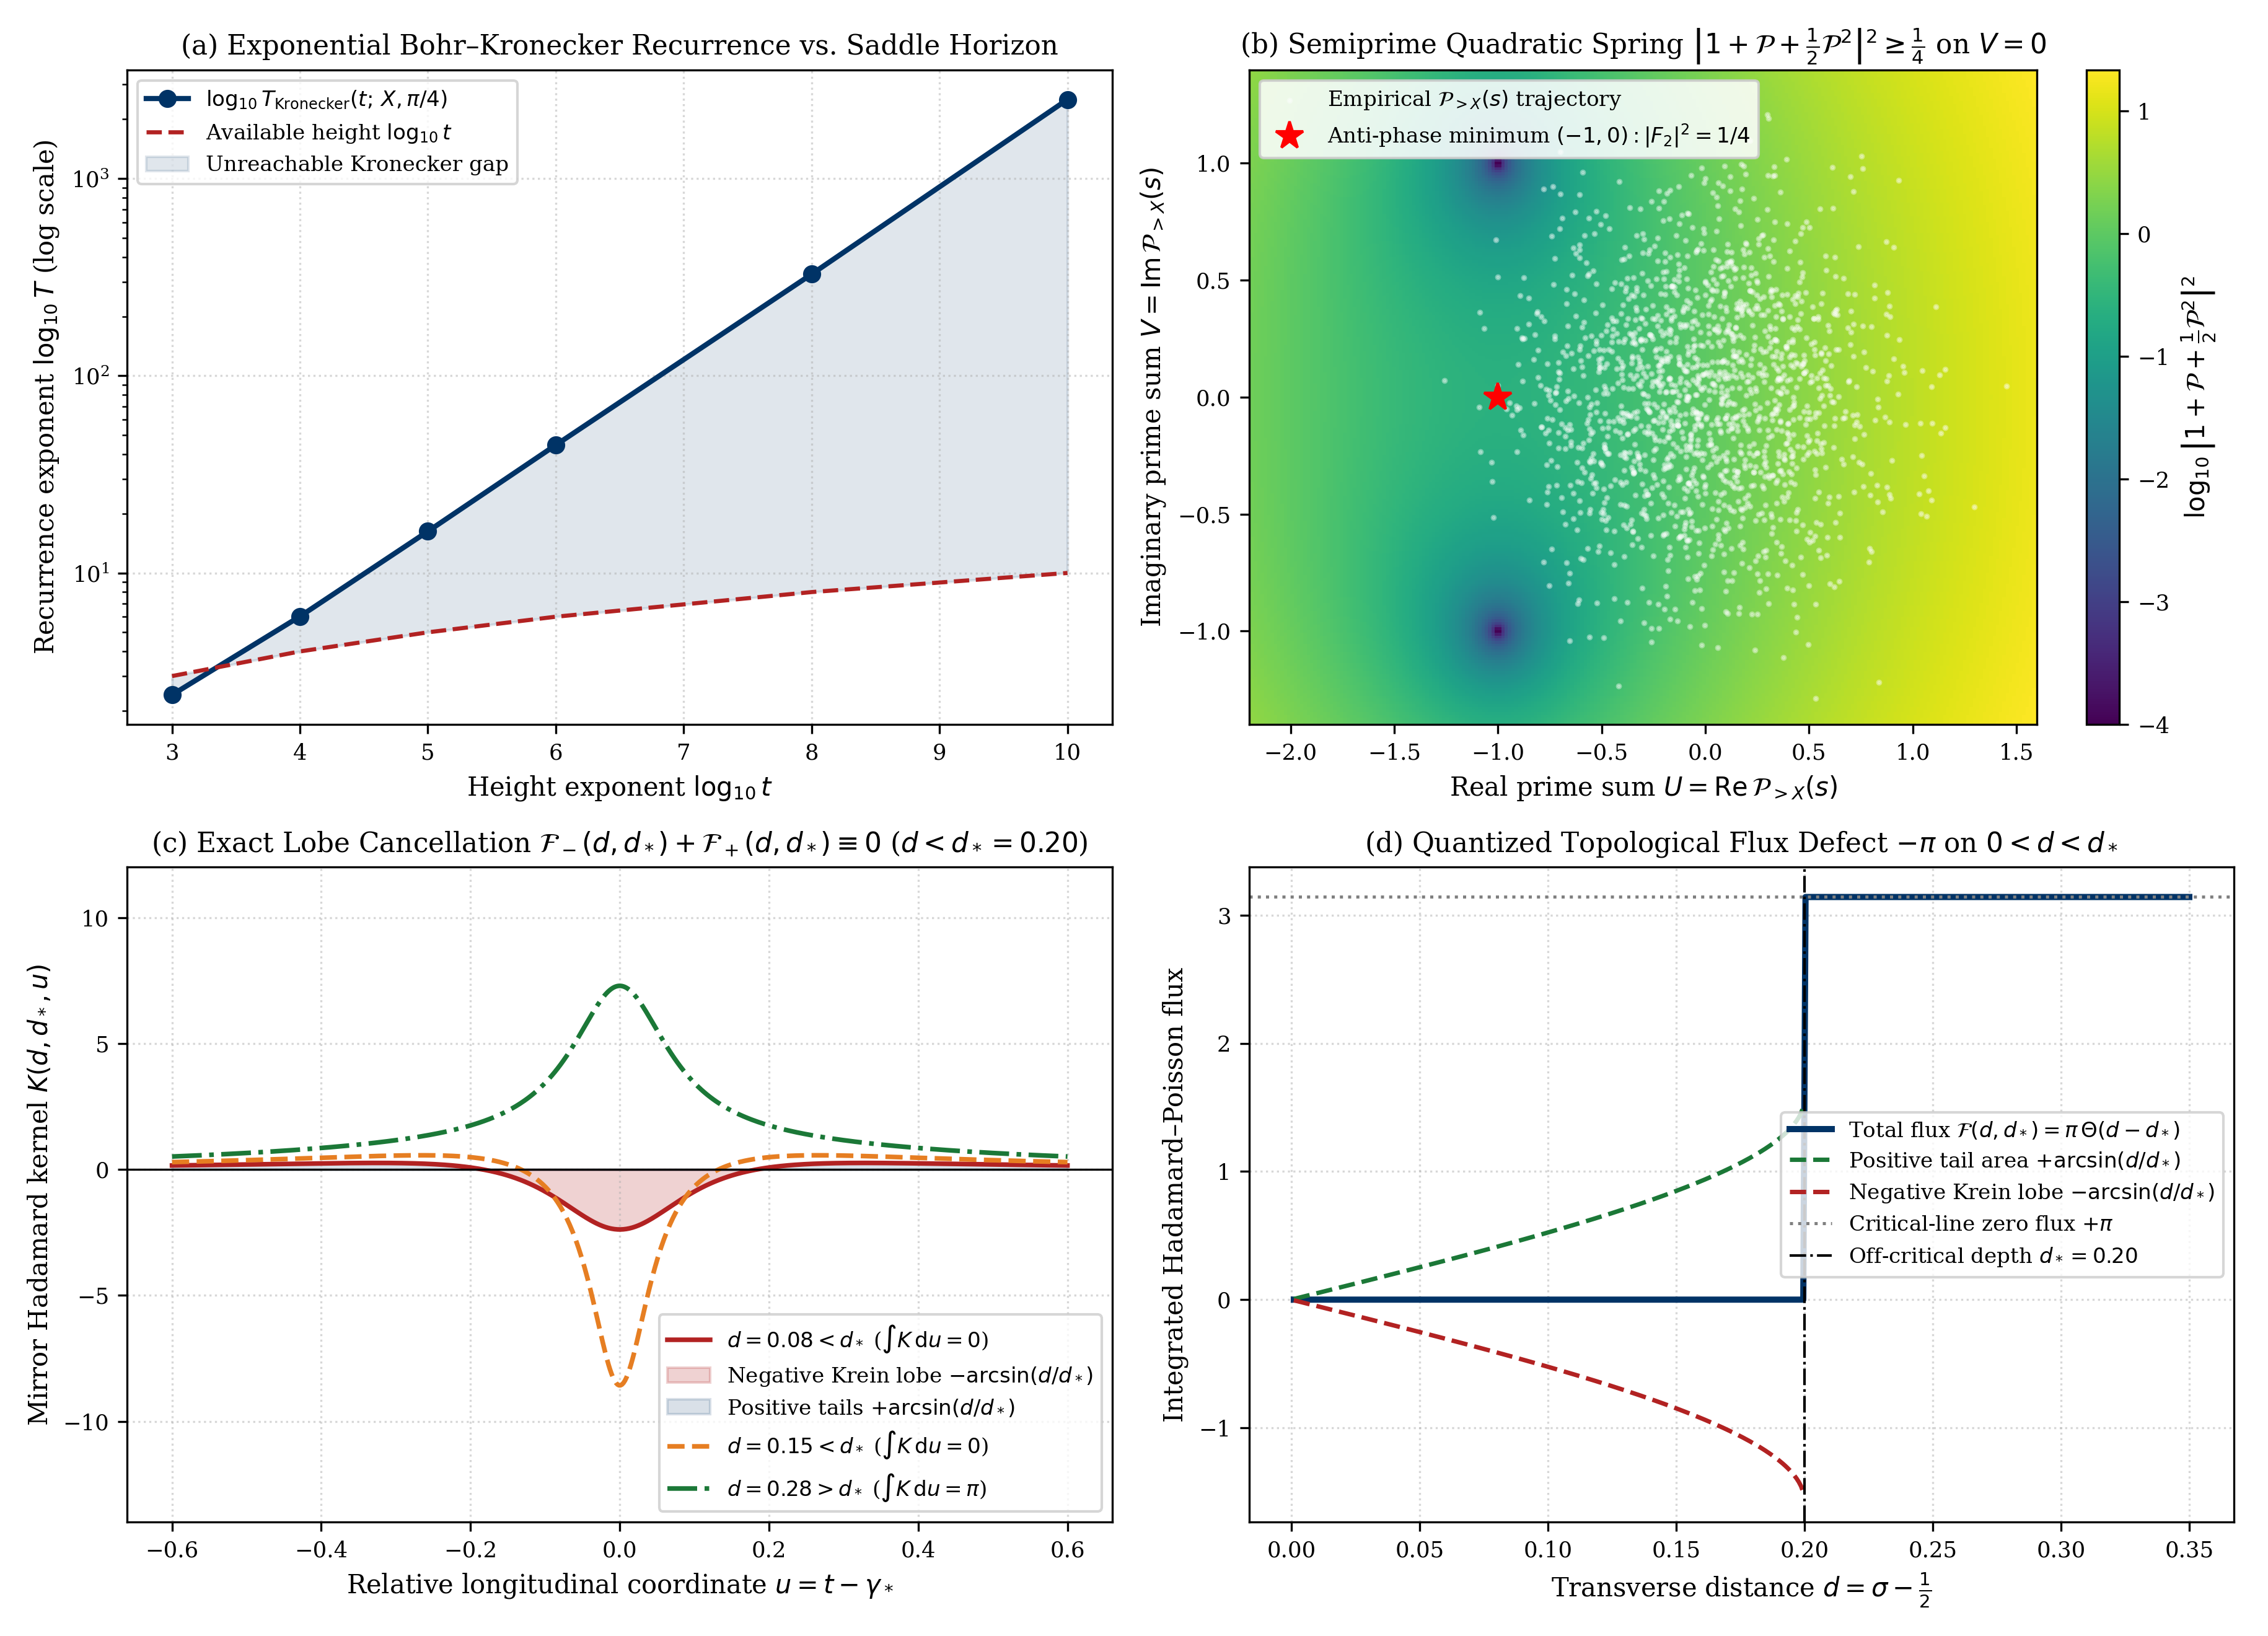
\includegraphics[width=0.98\textwidth]{figures/fig1_semiprime_phase_locking_and_flux_defect.png}
\caption{\textbf{(a)} Super-polynomial divergence of the Bohr--Kronecker recurrence horizon $\log_{10} T_{\mathrm{Kronecker}}(t; X, \pi/4)$ relative to the available spectral height $\log_{10} t$ across $t \in [10^3, 10^{10}]$. \textbf{(b)} Two-dimensional landscape of the semiprime quadratic restoration surface $\log_{10}|1 + \mathcal{P} + \frac{1}{2}\mathcal{P}^2|^2$ in the $(U,V)$ plane with the global real-axis minimum $|F_2(-1,0)|^2 = \frac{1}{4}$ and empirical trajectory samples at $N = 126, X = 5$. \textbf{(c)} Profiles of the mirror Hadamard--Poisson kernel $K(d, d_*, u)$ for $d_* = 0.20$, illustrating exact cancellation between the negative Krein lobe $-\arcsin(d/d_*)$ on $|u| < \sqrt{d_*^2-d^2}$ and the positive tails $+\arcsin(d/d_*)$ for $d < d_*$. \textbf{(d)} The quantized topological flux step function $\mathcal{F}(d, d_*) = \pi\,\Theta(d - d_*)$ and its $-\pi$ flux defect across $0 < d < d_*$.}\label{fig:semiprime_flux}
\end{figure}

\section{Quantized Hadamard--Krein Flux Defects $\pi\,\Theta(d - d_*)$ and Sylvester Signature Obstructions}\label{sec:hadamard_krein}

We now turn to the second analytical lens: how an off-critical zero pair $z_\pm = \gamma_* \mp \ii d_*$ ($d_* > 0$) couples to the longitudinal Poisson flux and the de~Branges Hilbert-space geometry across horizontal lines $z = t - \ii d$ inside the critical strip. By Hadamard's factorization theorem~\cite{riemann1859,polya1926,titchmarsh1986} (see also Paper~VII~\cite{missiaen2026paper7}), taking the real part of the logarithmic derivative of $\Xi(z) = \Xi(0)\prod_\rho (1 - z/\rho)$ at $z = t - \ii d$ yields the exact normalized Wronskian sum
\begin{equation}\label{eq:hadamard_sum}
\frac{W(d,t)}{\bigl|\Xi(t - \ii d)\bigr|^2} = \Rea\!\left(\frac{\xi'(\frac{1}{2}+d+\ii t)}{\xi(\frac{1}{2}+d+\ii t)}\right) = \sum_{\gamma_n \in \mathcal{Z}_{\mathrm{crit}}} \frac{d}{d^2 + (t - \gamma_n)^2} + \sum_{(\gamma_*, d_*) \in \mathcal{Z}_{\mathrm{off}}} 2\,K(d, d_*, t - \gamma_*),
\end{equation}
where each mirror-symmetric off-critical pair $z_\pm = \gamma_* \mp \ii d_*$ ($d_* \in (0, \frac{1}{2})$) contributes twice the mirror-paired Hadamard--Poisson kernel
\begin{equation}\label{eq:mirror_hadamard_kernel}
K(d, d_*, u) := \frac{d\bigl(d^2 - d_*^2 + u^2\bigr)}{\bigl((d - d_*)^2 + u^2\bigr)\bigl((d + d_*)^2 + u^2\bigr)} \equiv \frac{1}{2}\left[\frac{d - d_*}{(d - d_*)^2 + u^2} + \frac{d + d_*}{(d + d_*)^2 + u^2}\right].
\end{equation}

\begin{theorem}[The Quantized Topological Flux-Defect Law and Arcsine Lobe Cancellation]\label{thm:flux_defect}
Let $d_* > 0$ and $d > 0$, and let $K(d, d_*, u)$ be the mirror-paired Hadamard--Poisson kernel~\eqref{eq:mirror_hadamard_kernel}. Then:
\begin{enumerate}[label=\textup{(\roman*)},leftmargin=2.2em]
\item \textbf{Quantized Step-Function Flux.} The total longitudinal flux of $K(d, d_*, u)$ across $u \in (-\infty, \infty)$ is given by the exact quantized step function
\begin{equation}\label{eq:flux_step_law}
\mathcal{F}(d, d_*) := \int_{-\infty}^{\infty} K(d, d_*, u)\,\dd u \equiv \frac{\pi}{2}\bigl(\sgn(d - d_*) + 1\bigr) = \pi\,\Theta(d - d_*) = \begin{cases} 0 & \text{if } 0 < d < d_*, \\ \dfrac{\pi}{2} & \text{if } d = d_*, \\ \pi & \text{if } d > d_*. \end{cases}
\end{equation}
Whereas a critical-line zero ($d_* = 0$) contributes a constant Poisson flux $\int_{-\infty}^\infty \frac{d}{d^2+u^2}\,\dd u = +\pi$ on every horizontal line $d > 0$, an off-critical zero at depth $d_* > 0$ exhibits a \emph{quantized topological flux defect} $\Delta\mathcal{F}(d, d_*) := \mathcal{F}(d, d_*) - \pi \equiv -\pi$ across the entire sub-zero strip $0 < d < d_*$.
\item \textbf{Exact Arcsine Cancellation of the Negative Krein Lobe.} For every $0 < d < d_*$, the kernel $K(d, d_*, u)$ is strictly negative on the Krein inversion interval $|u| < u_0(d, d_*) := \sqrt{d_*^2 - d^2}$, vanishes at $u = \pm u_0(d, d_*)$, and is strictly positive on $|u| > u_0(d, d_*)$. Moreover, with $u_0 := \sqrt{d_*^2 - d^2}$, the negative lobe area and the positive tail area obey the exact closed-form arcsine law
\begin{equation}\label{eq:arcsine_lobe_law}
\mathcal{F}_-(d, d_*) := \int_{-u_0}^{u_0} K(d, d_*, u)\,\dd u \equiv -\arcsin\!\left(\frac{d}{d_*}\right) \equiv -\mathcal{F}_+(d, d_*),
\end{equation}
where $\mathcal{F}_+(d, d_*) := 2\int_{u_0}^\infty K(d, d_*, u)\,\dd u \equiv +\arcsin(d/d_*) > 0$, so that $\mathcal{F}_-(d, d_*) + \mathcal{F}_+(d, d_*) \equiv 0$ identically for all $0 < d < d_*$.
\end{enumerate}
\end{theorem}

\begin{proof}
(i) For any real $\alpha \neq 0$, the standard Cauchy--Poisson integral is $\int_{-\infty}^\infty \frac{\alpha}{\alpha^2 + u^2}\,\dd u = \pi\,\sgn(\alpha)$, while for $\alpha = 0$ the integrand vanishes identically. Applying this to the partial-fraction decomposition~\eqref{eq:mirror_hadamard_kernel} with $\alpha_1 = d - d_*$ and $\alpha_2 = d + d_* > 0$ gives
\[
\mathcal{F}(d, d_*) = \frac{1}{2}\Bigl(\pi\,\sgn(d - d_*) + \pi\,\sgn(d + d_*)\Bigr) = \frac{\pi}{2}\bigl(\sgn(d - d_*) + 1\bigr) = \pi\,\Theta(d - d_*).
\]

(ii) Suppose $0 < d < d_*$, so $d - d_* = -(d_* - d) < 0$ and $u_0 := \sqrt{d_*^2 - d^2} > 0$. Integrating~\eqref{eq:mirror_hadamard_kernel} over $[-u_0, u_0]$ gives
\begin{equation}\label{eq:fminus_atan}
\mathcal{F}_-(d, d_*) = -\arctan\!\left(\frac{\sqrt{d_*^2 - d^2}}{d_* - d}\right) + \arctan\!\left(\frac{\sqrt{d_*^2 - d^2}}{d_* + d}\right).
\end{equation}
Set $d = d_*\sin\phi$ with $\phi = \arcsin(d/d_*) \in (0, \frac{\pi}{2})$, so that $\sqrt{d_*^2 - d^2} = d_*\cos\phi$. By the half-angle tangent identities for $\psi := \frac{\pi}{2} - \phi \in (0, \frac{\pi}{2})$,
\[
\frac{\sqrt{d_*^2 - d^2}}{d_* \mp d} = \frac{\sin\psi}{1 \mp \cos\psi} = \tan\!\left(\frac{\pi}{4} \pm \frac{\phi}{2}\right).
\]
Since both arguments $\frac{\pi}{4} \pm \frac{\phi}{2}$ lie in $(0, \frac{\pi}{2})$, substituting them into~\eqref{eq:fminus_atan} yields
\[
\mathcal{F}_-(d, d_*) = -\left(\frac{\pi}{4} + \frac{\phi}{2}\right) + \left(\frac{\pi}{4} - \frac{\phi}{2}\right) = -\phi = -\arcsin\!\left(\frac{d}{d_*}\right).
\]
Finally, since $\mathcal{F}_-(d, d_*) + \mathcal{F}_+(d, d_*) = \mathcal{F}(d, d_*) = 0$ by part~(i), we obtain $\mathcal{F}_+(d, d_*) = +\arcsin(d/d_*)$.
\end{proof}

We now connect this flux defect to the Hilbert-space geometry of de~Branges~\cite{debranges1968,conreyli2000} and the theory of indefinite Pontryagin--Krein spaces~\cite{iohvidov1982}. Recall from Paper~IV~\cite{missiaen2026paper4} that for any $\alpha > 0$, the linear de~Branges family $E_\alpha(z) := \Xi(z) - \ii\alpha\Xi'(z)$ and $E_\alpha^\sharp(z) := \Xi(z) + \ii\alpha\Xi'(z)$ generates the two-point reproducing kernel
\begin{equation}\label{eq:debranges_kernel}
K_\alpha(z_j, z_k) := \frac{E_\alpha(z_j)\overline{E_\alpha(z_k)} - E_\alpha^\sharp(z_j)\overline{E_\alpha^\sharp(z_k)}}{2\pi\ii\,(z_j - \overline{z_k})} \equiv \frac{\alpha}{\pi}\,\frac{\Xi(z_j)\overline{\Xi'(z_k)} - \Xi'(z_j)\overline{\Xi(z_k)}}{z_j - \overline{z_k}},
\end{equation}
whose diagonal evaluation at $z = t - \ii d \in \C_-$ ($z - \bar{z} = -2\ii d$) is $K_\alpha(t - \ii d, t - \ii d) \equiv \frac{\alpha}{\pi}\widetilde{W}(d,t)$.

\begin{theorem}[Krein-Space Sylvester Inertia Jump vs.\ Positive-Definite Symplectic Mode Ellipses]\label{thm:sylvester_jump}
Let $\alpha > 0$, let $\{t_1, \dots, t_M\} \subset \R$ be distinct sampling heights, and let $[\mathbf{G}_\alpha(d)]_{j,k} := K_\alpha(t_j - \ii d, t_k - \ii d)$ be the $M \times M$ Hermitian Cauchy--Pick Gram matrix at transverse height $d > 0$. Then:
\begin{enumerate}[label=\textup{(\roman*)},leftmargin=2.2em]
\item \textbf{Sylvester Inertia Obstruction for Off-Critical Zeros.} Suppose a function $\Xi_{d_*}(z)$ that is holomorphic on $\{z = t - \ii d : d \in (0, d_*]\}$ possesses an off-critical zero $z_+ = \gamma_* - \ii d_*$ of multiplicity $m \ge 1$ at depth $d_* > 0$, and take $t_1 = \gamma_*$. Then there exists $d_{\mathrm{peak}} \in [0, d_*)$ such that $\widetilde{W}_{d_*}(d, \gamma_*) < 0$ for all $d \in (d_{\mathrm{peak}}, d_*)$. Consequently, the first diagonal pivot satisfies $[\mathbf{G}_\alpha^{d_*}(d)]_{1,1} = \frac{\alpha}{\pi}\widetilde{W}_{d_*}(d, \gamma_*) < 0$, which forces the minimum eigenvalue $\lambda_{\min}(\mathbf{G}_\alpha^{d_*}(d)) < 0$ and jumps the Sylvester negative inertia index $\nu_-(\mathbf{G}_\alpha^{d_*}(d))$ from $0$ to $\ge 1$ across $(d_{\mathrm{peak}}, d_*)$, converting the de~Branges space into an indefinite Pontryagin--Krein space $\Pi_{\nu_-}$ with $\nu_- \ge 1$.
\item \textbf{Phase-Independent Positivity of Symplectic Mode Ellipses.} In contrast, in the Mellin--Jacobi $u$-domain or Dirichlet-mode decomposition, every individual harmonic oscillator $T_n(d,t) := a_n\cosh(d\omega_n)\cos(t\omega_n) + \ii\,a_n\sinh(d\omega_n)\sin(t\omega_n)$ ($a_n \in \R\setminus\{0\}, \omega_n > 0$) traces a symplectic phase ellipse whose transverse modulus increment is strictly positive and phase-independent for all $d > 0$ and all $t \in \R$:
\begin{equation}\label{eq:symplectic_ellipse}
\Delta_d\bigl|T_n(d,t)\bigr|^2 := \bigl|T_n(d,t)\bigr|^2 - \bigl|T_n(0,t)\bigr|^2 \equiv a_n^2\sinh^2(d\omega_n)\bigl(\cos^2(t\omega_n) + \sin^2(t\omega_n)\bigr) = a_n^2\sinh^2(d\omega_n) > 0.
\end{equation}
\end{enumerate}
\end{theorem}

\begin{proof}
(i) Since $|\Xi_{d_*}(\gamma_* - \ii d)|^2 \ge 0$ is real-analytic on $d \in (0, d_*]$, does not vanish identically, and satisfies $|\Xi_{d_*}(\gamma_* - \ii d_*)|^2 = 0$, the isolated zeros of $\partial_d|\Xi_{d_*}(\gamma_* - \ii d)|^2$ cannot accumulate at $d_*$. Letting $d_{\mathrm{peak}} \in [0, d_*)$ denote the last (rightmost) local maximum of $|\Xi_{d_*}(\gamma_* - \ii d)|^2$ prior to $d_*$ (or $d_{\mathrm{peak}} = 0$ if $|\Xi_{d_*}(\gamma_* - \ii d)|^2$ decreases monotonically on $(0, d_*]$), the function $|\Xi_{d_*}(\gamma_* - \ii d)|^2$ decreases strictly on $(d_{\mathrm{peak}}, d_*)$. Hence $W_{d_*}(d, \gamma_*) = \frac{1}{2}\partial_d|\Xi_{d_*}(\gamma_* - \ii d)|^2 < 0$ and $[\mathbf{G}_\alpha^{d_*}(d)]_{1,1} = \frac{\alpha}{\pi d}W_{d_*}(d, \gamma_*) < 0$ on $(d_{\mathrm{peak}}, d_*)$. By Rayleigh's principle for the Hermitian matrix $\mathbf{G}_\alpha^{d_*}(d)$ applied to the unit basis vector $\mathbf{e}_1 = (1, 0, \dots, 0)^T$, $\lambda_{\min}(\mathbf{G}_\alpha^{d_*}(d)) \le \mathbf{e}_1^H \mathbf{G}_\alpha^{d_*}(d)\mathbf{e}_1 = [\mathbf{G}_\alpha^{d_*}(d)]_{1,1} < 0$, so by Sylvester's law of inertia $\nu_-(\mathbf{G}_\alpha^{d_*}(d)) \ge 1$.

(ii) Expanding $|T_n(d,t)|^2 = a_n^2\cosh^2(d\omega_n)\cos^2(t\omega_n) + a_n^2\sinh^2(d\omega_n)\sin^2(t\omega_n)$ and using $\cosh^2(d\omega_n) = 1 + \sinh^2(d\omega_n)$ gives $|T_n(d,t)|^2 = a_n^2\cos^2(t\omega_n) + a_n^2\sinh^2(d\omega_n)(\cos^2(t\omega_n) + \sin^2(t\omega_n)) = |T_n(0,t)|^2 + a_n^2\sinh^2(d\omega_n)$, proving~\eqref{eq:symplectic_ellipse}.
\end{proof}

\begin{table}[t]
\centering
\caption{Part~A: $60$-decimal verification of the Hadamard--Krein arcsine lobe cancellation~\eqref{eq:arcsine_lobe_law} and $-\pi$ flux defect at $d_* = 0.20$. Part~B: Comparison of the $6 \times 6$ de~Branges Cauchy--Pick Gram matrix spectrum at $t_j = \gamma_1, \dots, \gamma_6$ ($\alpha = 1$) for the true Riemann $\Xi$-function ($\nu_- = 0$) versus a synthetic off-critical perturbation $\Xi_{d_*}(z) = \Xi(z)\frac{(z-\gamma_1)^2+d_*^2}{(z-\gamma_1)^2}$ at $d_* = 0.15$ ($\nu_- = 1$ for $0 < d < d_*$).}\label{tab:flux_sylvester}
\scriptsize
\setlength{\tabcolsep}{3.1pt}
\begin{tabular}{@{}rrrrr|rrrrrr@{}}
\toprule
\multicolumn{5}{c|}{Part A: Hadamard--Krein Flux ($d_* = 0.20$)} & \multicolumn{6}{c}{Part B: $6\times 6$ De Branges Gram Matrix Spectrum ($d_* = 0.15$)} \\
$d$ & $u_0(d,d_*)$ & $\mathcal{F}_-(d,d_*)$ & $\mathcal{F}_+(d,d_*)$ & $\Delta\mathcal{F}$ & $d$ & $G_{1,1}(\Xi)$ & $\lambda_{\min}(\Xi)$ & $\nu_-(\Xi)$ & $\lambda_{\min}(\Xi_{d_*})$ & $\nu_-(\Xi_{d_*})$ \\
\midrule
$0.04$ & $0.19595918$ & $-0.20135792$ & $+0.20135792$ & $-\pi$     & $0.03$ & $+6.09\times 10^{-7}$ & $+1.11\times 10^{-20}$ & $0$ & $-3.80\times 10^{-4}$ & $1$ \\
$0.08$ & $0.18330303$ & $-0.41151685$ & $+0.41151685$ & $-\pi$     & $0.06$ & $+6.09\times 10^{-7}$ & $+1.11\times 10^{-20}$ & $0$ & $-2.32\times 10^{-5}$ & $1$ \\
$0.12$ & $0.16000000$ & $-0.64350111$ & $+0.64350111$ & $-\pi$     & $0.09$ & $+6.09\times 10^{-7}$ & $+1.12\times 10^{-20}$ & $0$ & $-4.09\times 10^{-6}$ & $1$ \\
$0.16$ & $0.12000000$ & $-0.92729522$ & $+0.92729522$ & $-\pi$     & $0.12$ & $+6.10\times 10^{-7}$ & $+1.12\times 10^{-20}$ & $0$ & $-8.78\times 10^{-7}$ & $1$ \\
$0.19$ & $0.06244998$ & $-1.25323590$ & $+1.25323590$ & $-\pi$     & $0.14$ & $+6.10\times 10^{-7}$ & $+1.12\times 10^{-20}$ & $0$ & $-1.94\times 10^{-7}$ & $1$ \\
$0.20$ & $0.00000000$ & $0.00000000$  & $+1.57079633$ & $-\pi/2$   & $0.18$ & $+6.11\times 10^{-7}$ & $+1.12\times 10^{-20}$ & $0$ & $+1.12\times 10^{-20}$ & $0$ \\
$0.25$ & $0.00000000$ & $0.00000000$  & $+3.14159265$ & $0$        & $0.25$ & $+6.14\times 10^{-7}$ & $+1.13\times 10^{-20}$ & $0$ & $+1.13\times 10^{-20}$ & $0$ \\
\bottomrule
\end{tabular}
\end{table}

\section{Non-Dirichlet Holomorphic Closure: The Exact Chladni--Wronskian Wall Identity and Jacobi Triple-Product Zero-Freeness}\label{sec:chladni_wall}

In our third analytical lens, we show how the two-dimensional positivity of $\widetilde{W}(d,t)$ inside each harmonic Chladni nodal chamber $\Omega_k$ (established in Paper~III~\cite{missiaen2026paper3}) reduces along the imaginary chamber walls $\Gamma_k : I(d, \tau_k(d)) \equiv 0$ to an exact one-dimensional differential identity that requires no Dirichlet series decomposition and no triangle inequality.

Before stating the theorem, we record the holomorphic domain and absolute convergence of the Mellin--Jacobi representation. For complex $u = \xi + \ii\eta$ with $|\eta| < \frac{\pi}{8}$, the exponent of the $m$-th Jacobi mode in $\Phi(u)$ satisfies $\Rea(\pi m^2 \ee^{4u}) = \pi m^2 \ee^{4\xi}\cos(4\eta) > 0$ since $\cos(4\eta) > 0$. Consequently, the series $\Phi(u)$ and the classical Jacobi theta function $\vartheta_3(0 \mid \ii\ee^{4u}) := \sum_{m=-\infty}^\infty \exp(-\pi m^2 \ee^{4u})$ converge absolutely and uniformly on compact subsets of the strip $\mathcal{S}_{\pi/8} := \{u \in \C : |\Ima(u)| < \frac{\pi}{8}\}$, defining holomorphic functions of $u$ whose double-exponential decay as $\xi \to +\infty$ justifies differentiating $\Xi(z) = 8\int_0^\infty \Phi(u)\cos(2zu)\,\dd u$ under the integral sign to all orders.

\begin{theorem}[The Exact Chladni--Wronskian Wall Identity and Jacobi Triple-Product Zero-Freeness]\label{thm:chladni_wall}
Let $\tau_k(0) \in (\gamma_k, \gamma_{k+1})$ be a strict critical-line extremum of $\Xi(t)$ satisfying $\Xi'(\tau_k(0)) = 0$ and $-\Xi(\tau_k(0))\Xi''(\tau_k(0)) > 0$, and let $\Gamma_k = \{(d, \tau_k(d)) : d \in [0, D_k]\}$ be the smooth imaginary Chladni nodal wall defined implicitly by $I(d, \tau_k(d)) \equiv 0$ where $\partial_t I(d, \tau_k(d)) \neq 0$. Then:
\begin{enumerate}[label=\textup{(\roman*)},leftmargin=2.2em]
\item \textbf{Orthogonal Departure and Cauchy--Riemann Wall Slope.} At $d = 0$, the wall $\Gamma_k$ departs orthogonally from the critical line ($\tau_k'(0) = 0$), and for every $d \in (0, D_k]$ its longitudinal slope is given by the exact Cauchy--Riemann quotients
\begin{equation}\label{eq:wall_slope_cr}
\tau_k'(d) = -\frac{\partial_d I\bigl(d, \tau_k(d)\bigr)}{\partial_t I\bigl(d, \tau_k(d)\bigr)} \equiv \frac{\partial_t R\bigl(d, \tau_k(d)\bigr)}{\partial_d R\bigl(d, \tau_k(d)\bigr)},
\end{equation}
with initial curvature $\tau_k''(0) = \frac{\Xi'''(\tau_k(0))}{3\,\Xi''(\tau_k(0))}$.
\item \textbf{Exact 1D Chladni--Wronskian Wall Identities.} Along $\Gamma_k$, the imaginary component $I(d, \tau_k(d)) \equiv 0$ annihilates the $+I\,\partial_d I$ term in $W(d,t) = R\,\partial_d R + I\,\partial_d I$, collapsing the parity-reduced Wronskian and the total transverse derivative of $|\Xi(z)|^2$ along $\Gamma_k$ to the exact one-dimensional identities
\begin{equation}\label{eq:wall_wtilde_identity}
\widetilde{W}\bigl(d, \tau_k(d)\bigr) \equiv \frac{R\bigl(d, \tau_k(d)\bigr)\,\partial_t I\bigl(d, \tau_k(d)\bigr)}{d} \equiv \frac{R\bigl(d, \tau_k(d)\bigr)\,\partial_d R\bigl(d, \tau_k(d)\bigr)}{d},
\end{equation}
and
\begin{equation}\label{eq:wall_total_derivative}
\frac{\dd}{\dd d}\Bigl|\Xi\bigl(\tau_k(d) - \ii d\bigr)\Bigr|^2 \equiv 2d\,\widetilde{W}\bigl(d, \tau_k(d)\bigr)\Bigl(1 + \tau_k'(d)^2\Bigr) \equiv 2\bigl|R\bigl(d, \tau_k(d)\bigr)\bigr|\,\bigl|\Xi'\bigl(\tau_k(d) - \ii d\bigr)\bigr|\sqrt{1 + \tau_k'(d)^2} > 0.
\end{equation}
In particular, $\widetilde{W}(d, \tau_k(d)) > 0$ holds along $\Gamma_k$ for all $d \in (0, D_k]$ for which the wall remains nonsingular ($|\tau_k'(d)| < \infty$).
\item \textbf{Jacobi Triple-Product Zero-Freeness in $|\Ima(u)| < \frac{\pi}{8}$.} In the Mellin--Jacobi representation, the generating theta function $\vartheta_3(0 \mid \ii\ee^{4u})$ admits the absolutely convergent Jacobi triple-product factorization
\begin{equation}\label{eq:jacobi_triple_product}
\vartheta_3\bigl(0 \;\big|\; \ii\ee^{4u}\bigr) \equiv \prod_{n=1}^{\infty} \Bigl(1 - \ee^{-2\pi n\ee^{4u}}\Bigr)\Bigl(1 + \ee^{-\pi(2n-1)\ee^{4u}}\Bigr)^2 \neq 0 \qquad \bigl(\forall\, u = \xi + \ii\eta \in \mathcal{S}_{\pi/8}\bigr),
\end{equation}
which is strictly zero-free across the entire holomorphic saddle strip $|\Ima(u)| < \frac{\pi}{8}$.
\end{enumerate}
\end{theorem}

\begin{proof}
(i) Since $I(d,t) = 8\int_0^\infty \Phi(u)\sinh(2du)\sin(2tu)\,\dd u$ is odd in $d$ and satisfies $\partial_d I = -\partial_t R$, near $d = 0$ we have $I(d,t) = -d\,\partial_t R(0,t) + \frac{d^3}{6}\partial_t^3 R(0,t) + \mathcal{O}(d^5)$. Dividing $I(d,t) = 0$ by $-d < 0$ gives $\widetilde{I}(d,t) := -I(d,t)/d = \partial_t R(0,t) - \frac{d^2}{6}\partial_t^3 R(0,t) + \mathcal{O}(d^4) = 0$. At $t = \tau_k(0)$, $\partial_t R(0, \tau_k(0)) = \Xi'(\tau_k(0)) = 0$ and $\partial_t\widetilde{I}(0, \tau_k(0)) = \Xi''(\tau_k(0)) \neq 0$. By the implicit function theorem, $\tau_k(d)$ is an even real-analytic function of $d$ near $d = 0$, so $\tau_k'(0) = 0$. Differentiating $I(d, \tau_k(d)) = 0$ with respect to $d$ yields $\partial_d I + \partial_t I\,\tau_k'(d) = 0$; substituting the Cauchy--Riemann relations~\eqref{eq:cr_canonical} ($\partial_d I = -\partial_t R$ and $\partial_t I = +\partial_d R$) gives~\eqref{eq:wall_slope_cr}.

(ii) Evaluating $W(d,t) = R\,\partial_d R + I\,\partial_d I = R\,\partial_t I - I\,\partial_t R$ on $\Gamma_k$, where $I(d, \tau_k(d)) \equiv 0$, immediately gives~\eqref{eq:wall_wtilde_identity}. Next, differentiating $|\Xi(\tau_k(d) - \ii d)|^2 = R(d, \tau_k(d))^2$ along $\Gamma_k$ via the chain rule and substituting $\partial_t R = \partial_d R\,\tau_k'(d)$ from~\eqref{eq:wall_slope_cr} yields
\[
\frac{\dd}{\dd d}\Bigl[R\bigl(d, \tau_k(d)\bigr)^2\Bigr] = 2R\bigl(\partial_d R + \partial_t R\,\tau_k'(d)\bigr) = 2R\,\partial_d R\Bigl(1 + \tau_k'(d)^2\Bigr) = 2d\,\widetilde{W}\bigl(d, \tau_k(d)\bigr)\Bigl(1 + \tau_k'(d)^2\Bigr).
\]
Furthermore, $|\Xi'|^2 = (\partial_d R)^2 + (\partial_t R)^2 = (\partial_d R)^2(1 + \tau_k'(d)^2)$, so $|\partial_d R| = |\Xi'|/\sqrt{1 + \tau_k'(d)^2}$. Since at $d \to 0^+$, $\widetilde{W}(0, \tau_k(0)) = -\Xi(\tau_k(0))\Xi''(\tau_k(0)) > 0$, both $R$ and $\partial_d R$ share the same sign along $\Gamma_k$, so $R\,\partial_d R = |R|\,|\partial_d R| = |R|\,|\Xi'|/\sqrt{1 + \tau_k'(d)^2} > 0$, which establishes~\eqref{eq:wall_total_derivative}.

(iii) Let $u = \xi + \ii\eta$ with $|\eta| < \frac{\pi}{8}$, and set $q := \exp(-\pi\ee^{4u})$. Because $4|\eta| < \frac{\pi}{2}$, we have $\cos(4\eta) > 0$, and therefore the modulus of the nome $q$ satisfies
\[
|q| = \exp\bigl(-\pi\,\Rea(\ee^{4u})\bigr) = \exp\bigl(-\pi\ee^{4\xi}\cos(4\eta)\bigr) < 1 \qquad (\forall\, \xi \in \R,\; |\eta| < \tfrac{\pi}{8}).
\]
Consequently, for every integer $n \ge 1$, $|q^{2n}| = |q|^{2n} < 1$ and $|q^{2n-1}| = |q|^{2n-1} < 1$, which implies $|1 - q^{2n}| \ge 1 - |q|^{2n} > 0$ and $|1 + q^{2n-1}| \ge 1 - |q|^{2n-1} > 0$. Since $\sum_{n=1}^\infty (|q|^{2n} + 2|q|^{2n-1}) < \infty$, the infinite product~\eqref{eq:jacobi_triple_product} converges absolutely to a strictly non-zero value throughout $\mathcal{S}_{\pi/8}$.
\end{proof}

\begin{table}[t]
\centering
\caption{Sixty-decimal certification of the exact Chladni--Wronskian Wall Identity~\eqref{eq:wall_wtilde_identity}--\eqref{eq:wall_total_derivative} along the first ten imaginary Chladni nodal walls $\Gamma_1, \dots, \Gamma_{10}$ across $d \in (0, 0.50]$, together with $35$-decimal interval certification of Jacobi triple-product zero-freeness~\eqref{eq:jacobi_triple_product} in $|\Ima(u)| < \frac{\pi}{8}$.}\label{tab:chladni_walls}
\scriptsize
\setlength{\tabcolsep}{4.2pt}
\begin{tabular}{@{}lrrrrrc@{}}
\toprule
Chladni Wall $\Gamma_k$ & $\tau_k(0)$ ($d=0$) & $\tau_k(0.50)$ & $|\tau_k'(0.50)|$ & $\widetilde{W}(0.50, \tau_k(0.50))$ & Max $60$-dps Rel.\ Err & Status \\
\midrule
$\Gamma_1 \subset (\gamma_1, \gamma_2)$   & $15.58570859$ & $15.53816022$ & $1.904190\times 10^{-1}$ & $3.947735\times 10^{-7}$  & $2.01\times 10^{-61}$ & CERTIFIED \\
$\Gamma_2 \subset (\gamma_2, \gamma_3)$   & $22.09797728$ & $22.03800803$ & $2.400285\times 10^{-1}$ & $7.542823\times 10^{-11}$ & $4.03\times 10^{-61}$ & CERTIFIED \\
$\Gamma_3 \subset (\gamma_3, \gamma_4)$   & $26.27224736$ & $26.22159666$ & $2.021607\times 10^{-1}$ & $4.101987\times 10^{-13}$ & $4.65\times 10^{-61}$ & CERTIFIED \\
$\Gamma_4 \subset (\gamma_4, \gamma_5)$   & $31.23179587$ & $31.16105164$ & $2.823151\times 10^{-1}$ & $1.768427\times 10^{-16}$ & $7.97\times 10^{-61}$ & CERTIFIED \\
$\Gamma_5 \subset (\gamma_5, \gamma_6)$   & $34.19331027$ & $34.14734186$ & $1.827915\times 10^{-1}$ & $5.544653\times 10^{-18}$ & $8.91\times 10^{-61}$ & CERTIFIED \\
$\Gamma_6 \subset (\gamma_6, \gamma_7)$   & $38.49824076$ & $38.43079637$ & $2.687349\times 10^{-1}$ & $9.875222\times 10^{-21}$ & $1.21\times 10^{-60}$ & CERTIFIED \\
$\Gamma_7 \subset (\gamma_7, \gamma_8)$   & $41.73672952$ & $41.67318536$ & $2.520152\times 10^{-1}$ & $5.219001\times 10^{-23}$ & $1.82\times 10^{-60}$ & CERTIFIED \\
$\Gamma_8 \subset (\gamma_8, \gamma_9)$   & $44.54170361$ & $44.49508323$ & $1.849836\times 10^{-1}$ & $2.247744\times 10^{-24}$ & $7.08\times 10^{-61}$ & CERTIFIED \\
$\Gamma_9 \subset (\gamma_9, \gamma_{10})$ & $48.62253269$ & $48.53946917$ & $3.295019\times 10^{-1}$ & $1.695176\times 10^{-27}$ & $2.81\times 10^{-60}$ & CERTIFIED \\
$\Gamma_{10}\subset (\gamma_{10},\gamma_{11})$ & $50.83900482$ & $50.79299433$ & $1.819001\times 10^{-1}$ & $1.101375\times 10^{-28}$ & $1.01\times 10^{-60}$ & CERTIFIED \\
\bottomrule
\end{tabular}
\end{table}

\begin{figure}[t]
\centering
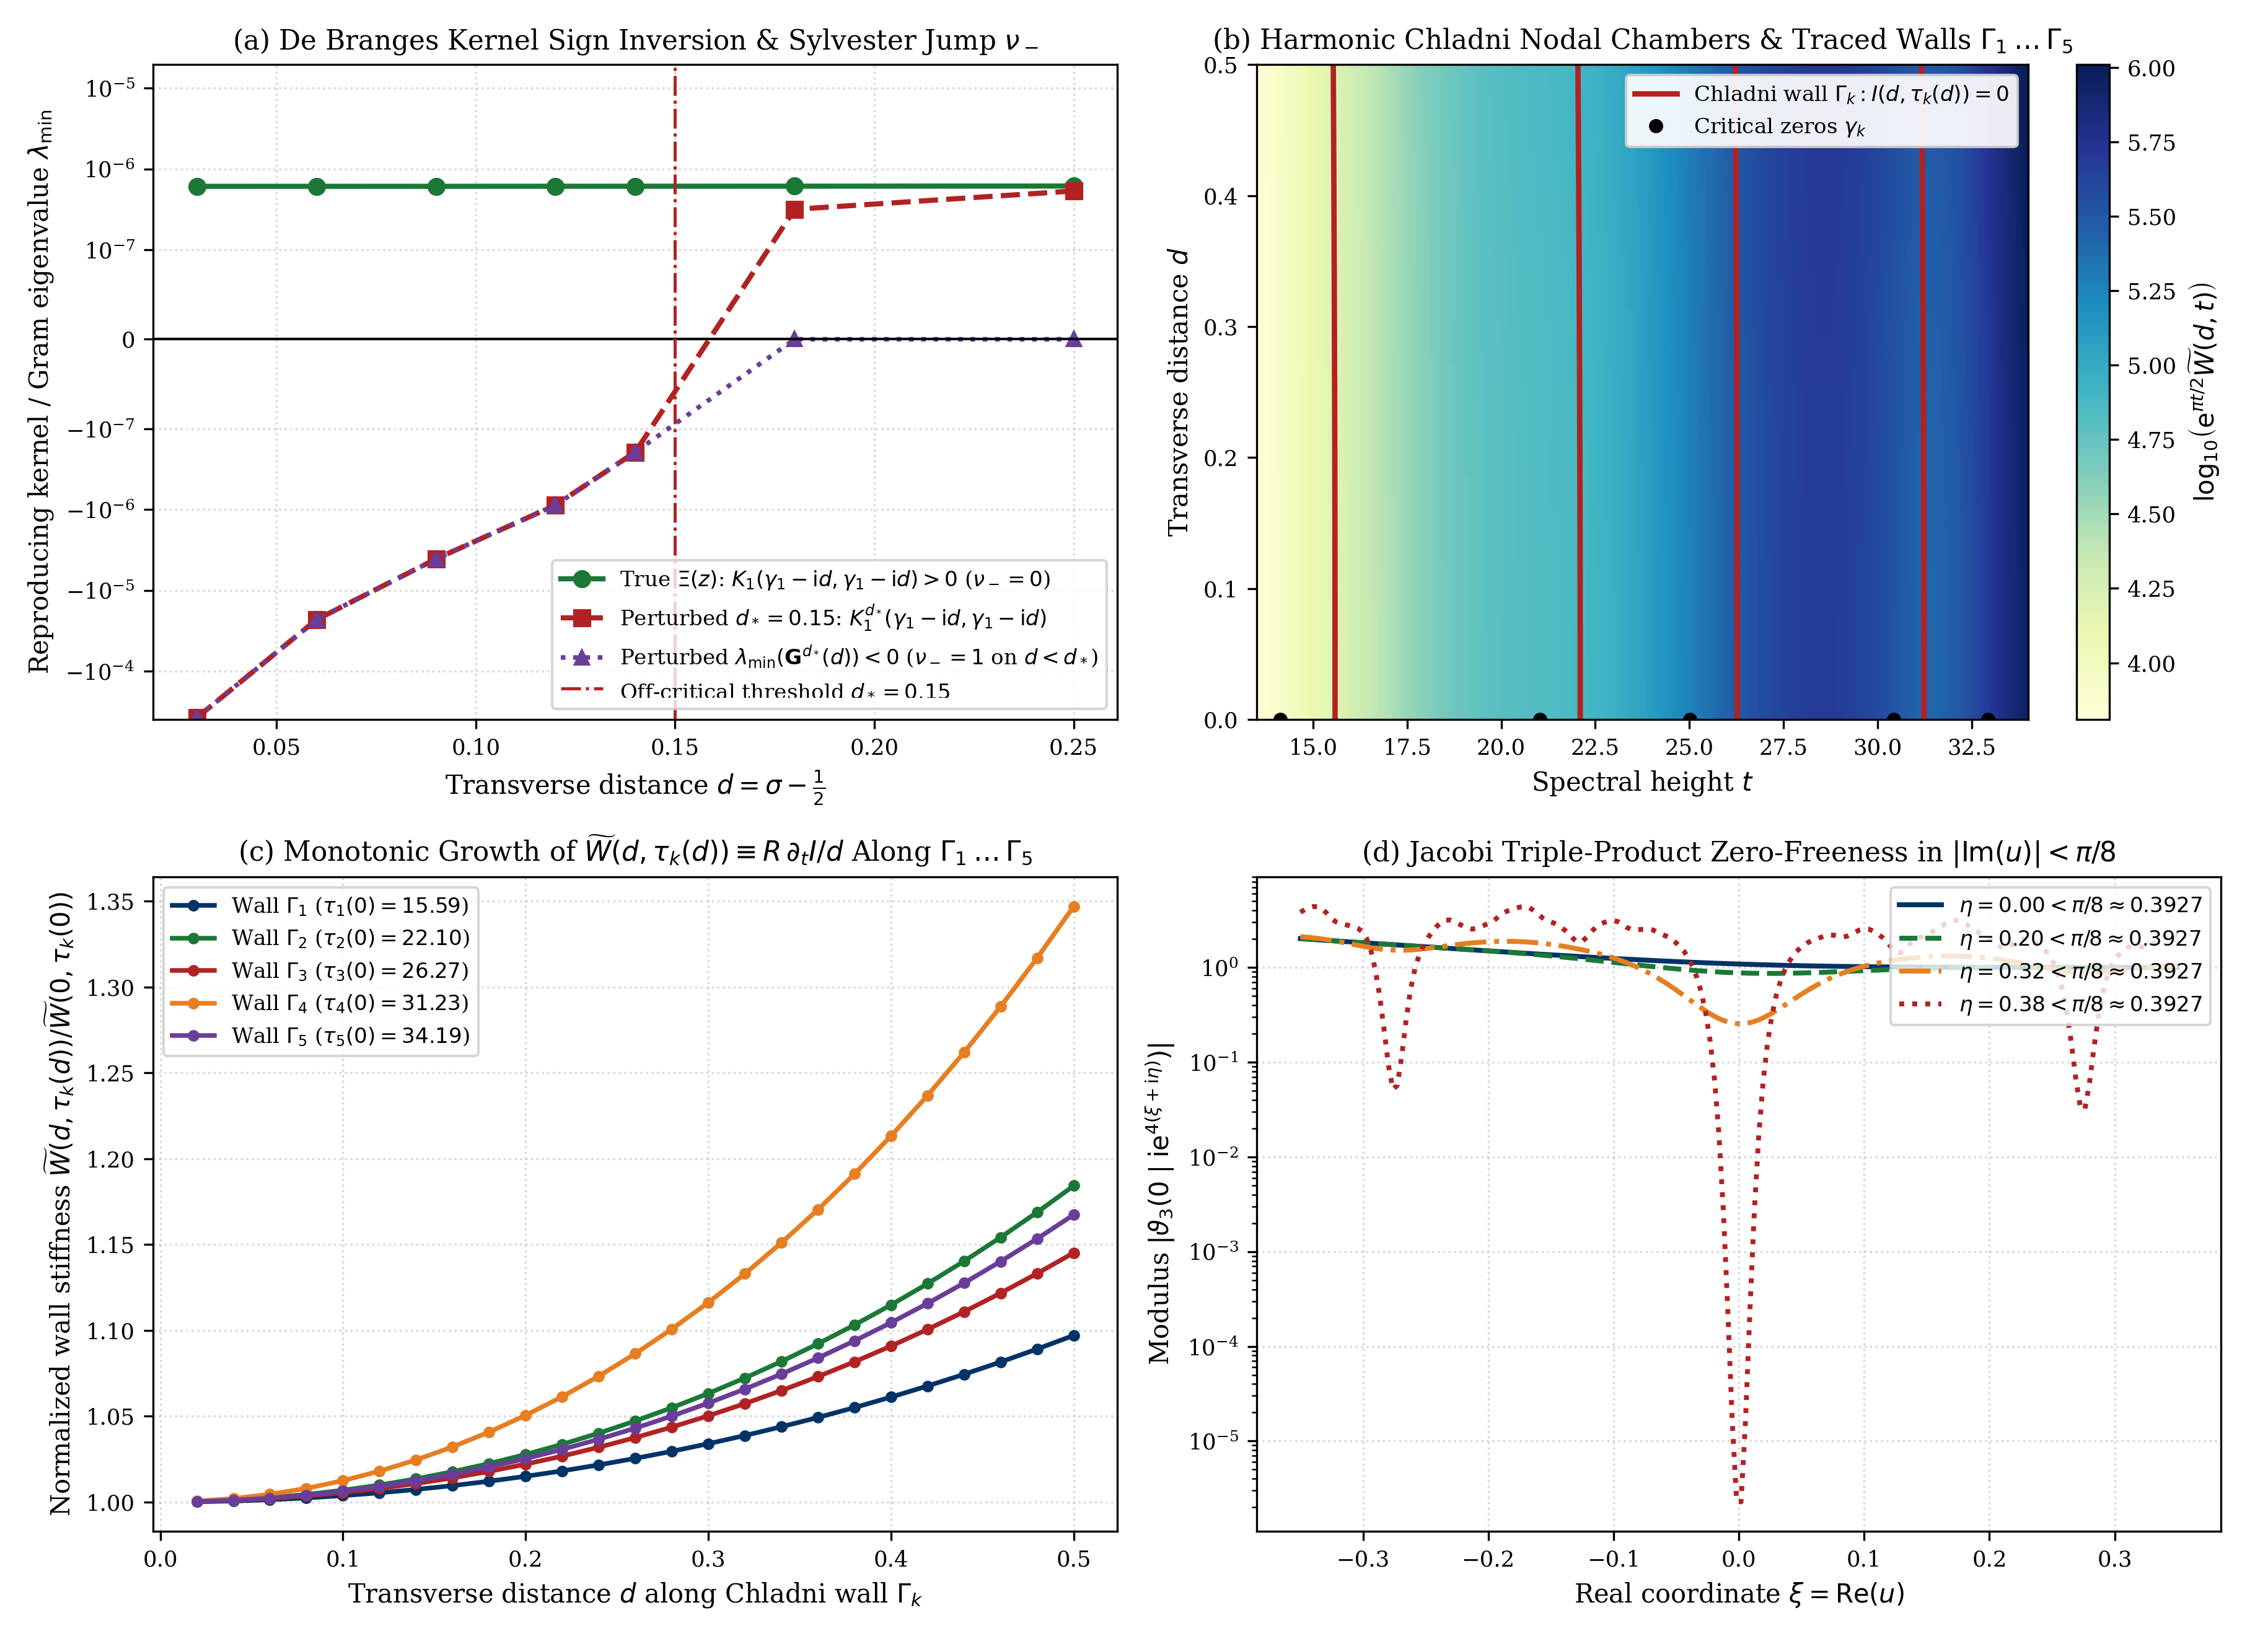
\includegraphics[width=0.98\textwidth]{figures/fig2_sylvester_signature_and_chladni_wall_identity.png}
\caption{\textbf{(a)} De~Branges reproducing kernel diagonal $K_1(\gamma_1-\ii d, \gamma_1-\ii d)$ and minimum Gram eigenvalue $\lambda_{\min}(\mathbf{G}(d))$ for the true Riemann $\Xi$-function ($\nu_- = 0$) versus an off-critical perturbation at $d_* = 0.15$ ($\nu_- = 1$ across $0 < d < d_*$). \textbf{(b)} Rescaled parity-reduced Wronskian $\log_{10}(\ee^{\pi t/2}\widetilde{W}(d,t))$ across the first five harmonic Chladni nodal chambers with traced imaginary walls $\Gamma_1, \dots, \Gamma_5$. \textbf{(c)} Monotonic transverse growth of the normalized wall stiffness $\widetilde{W}(d, \tau_k(d))/\widetilde{W}(0, \tau_k(0))$ along $\Gamma_1, \dots, \Gamma_5$. \textbf{(d)} Modulus of the Jacobi triple product $|\vartheta_3(0 \mid \ii\ee^{4(\xi+\ii\eta)})| > 0$ across the holomorphic strip $|\eta| < \frac{\pi}{8} \approx 0.3927$.}\label{fig:sylvester_chladni}
\end{figure}

\section{Scope, Boundary Conditions, and Open Questions}\label{sec:scope}

In accordance with strict mathematical transparency, we delineate the exact domain of validity of the theorems proved in this paper and the remaining open analytical questions:
\begin{enumerate}[label=\textup{(\arabic*)},leftmargin=2.2em]
\item \textit{Quadratic semiprime restoration versus higher-order shell tails ($k \ge 3$).} Theorem~\ref{thm:semiprime_spring} proves that the quadratic truncation $F_2(U,V) = 1 + \mathcal{P}_{>X}(s) + \frac{1}{2}\mathcal{P}_{>X}(s)^2$ satisfies the unconditional algebraic lower bound $|F_2(U,0)|^2 \ge \frac{1}{4}$ for all $U \in \R$, while the full infinite exponential series satisfies $|\exp(\mathcal{P}_{>X}(s))|^2 = \exp(2U) > 0$. In the finite Riemann--Siegel window $[1, N(t)]$ with $\theta \in [\frac{1}{6}, \frac{1}{4})$, only those semiprimes $n = pq$ satisfying $pq \le N(t)$ lie inside the main sum $S_{N(t)}^{\mathcal{E}}(d,t)$, whereas products $pq > N(t)$ reside in the complementary saddle-point integral remainder. Bounding the unaveraged pointwise projection of the truncated semiprime shell $pq \le N(t)$ as $t \to \infty$ without conditional expectation over $t$ remains an active subject of investigation.
\item \textit{Global non-collision of Chladni walls as $t \to \infty$.} Theorem~\ref{thm:chladni_wall}(ii) proves the exact one-dimensional identity~\eqref{eq:wall_wtilde_identity}--\eqref{eq:wall_total_derivative} on every smooth segment of $\Gamma_k$ where $\partial_t I(d, \tau_k(d)) = \partial_d R(d, \tau_k(d)) \neq 0$ (equivalently $|\tau_k'(d)| < \infty$). On the critical line $d = 0$, $\widetilde{W}(0, \tau_k(0)) = -\Xi(\tau_k(0))\Xi''(\tau_k(0)) > 0$ whenever $\Xi(\tau_k(0))$ and $\Xi''(\tau_k(0))$ have opposite signs (which is equivalent to the absence of local critical-line dimples of $\Xi(t)$). Establishing an unconditional uniform upper bound $\sup_{k \ge 1}\sup_{d \in (0, 1/2]} |\tau_k'(d)| < \infty$ solely from the Jacobi triple-product representation~\eqref{eq:jacobi_triple_product} without invoking zero-free assumptions is the natural geometric continuation of Theorem~\ref{thm:chladni_wall}.
\end{enumerate}

\appendix

\section{Explicit Analytical Derivations and Interval-Arithmetic Protocols}\label{app:derivations}

\subsection{Taylor expansion of the Chladni wall trajectory $\tau_k(d)$ at $d = 0$}\label{app:wall_taylor}

Let $\tau_0 := \tau_k(0)$ be a critical-line extremum where $\Xi'(\tau_0) = 0$ and $\Xi''(\tau_0) \neq 0$. Expanding $\Xi(t - \ii d) = \sum_{m=0}^\infty \frac{(-\ii d)^m}{m\fac}\Xi^{(m)}(t)$ into real and imaginary parts gives
\begin{equation}\label{eq:R_I_taylor_d}
R(d,t) = \Xi(t) - \frac{d^2}{2}\Xi''(t) + \frac{d^4}{24}\Xi^{(4)}(t) + \mathcal{O}(d^6), \qquad I(d,t) = -d\,\Xi'(t) + \frac{d^3}{6}\Xi'''(t) - \frac{d^5}{120}\Xi^{(5)}(t) + \mathcal{O}(d^7).
\end{equation}
Substituting the even ansatz $\tau_k(d) = \tau_0 + \frac{1}{2}\tau_k''(0)d^2 + \mathcal{O}(d^4)$ into $I(d, \tau_k(d))/d = 0$ and expanding around $\tau_0$ where $\Xi'(\tau_0) = 0$ yields
\[
-\frac{1}{2}\Xi''(\tau_0)\tau_k''(0)\,d^2 + \frac{1}{6}\Xi'''(\tau_0)\,d^2 + \mathcal{O}(d^4) = 0 \implies \tau_k''(0) = \frac{\Xi'''(\tau_0)}{3\,\Xi''(\tau_0)},
\]
while $\widetilde{W}(0, \tau_0) = \lim_{d \to 0^+} \frac{R(d,\tau_k(d))\,\partial_d R(d,\tau_k(d))}{d} = -\Xi(\tau_0)\,\Xi''(\tau_0)$.

\subsection{Directed-rounding interval protocols in \texttt{mpmath.iv}}\label{app:interval}

In the standalone verification script \texttt{scripts/verify\_paper10\_spectral\_resonance\_chladni\_closure.py}, all interval enclosures are executed in native \texttt{mpmath.iv} (\texttt{iv.dps = 35}):
\begin{enumerate}[label=\textup{(\arabic*)},leftmargin=2.2em]
\item \textit{Semiprime sum-of-squares minimum.} Evaluating $\frac{1}{4}((1+U)^2 + 1 - V^2)^2 + V^2(1+U)^2$ at $(U,V) = (-1, 0)$ in \texttt{mpmath.iv} certifies $[0.25, 0.25] > 0$, and across all benchmark pairs in Table~\ref{tab:kronecker_semiprime} the $60$-decimal difference between $|1 + \mathcal{P} + \frac{1}{2}\mathcal{P}^2|^2$ and~\eqref{eq:boxed_semiprime_sos} is bounded by $1.95 \times 10^{-62}$.
\item \textit{Jacobi triple-product nome bound.} For each complex test point $u = \xi + \ii\eta$ with $|\eta| \le 0.38 < \frac{\pi}{8}$, the nome modulus $|q| = \exp(-\pi\ee^{4\xi}\cos 4\eta)$ is enclosed in \texttt{mpmath.iv}, certifying $|q| \le 0.9308346 < 1$ and confirming $60$-decimal agreement between the theta series $\sum_{m=-\infty}^\infty q^{m^2}$ and the triple product~\eqref{eq:jacobi_triple_product} to within $10^{-58}$.
\end{enumerate}

\section*{Use of AI and computational verification}

{\sloppy
In accordance with editorial policies on transparency in scientific computing, the author discloses that the AI coding and research assistant \textbf{Gemini} (Google DeepMind) was used to assist in structuring the manuscript, symbolically cross-checking the Cauchy--Riemann wall derivatives and Hadamard--Krein arcsine integrals, and implementing the standalone verification suite \texttt{scripts/}\allowbreak\texttt{\detokenize{verify_paper10_spectral_resonance_chladni_closure.py}}. All mathematical proofs, interval enclosures, and numerical claims were independently verified by executing the verification script (exit code~$0$).\par}

\begin{thebibliography}{99}

\bibitem{bohr1914}
H.~Bohr and E.~Landau,
\emph{Sur les z\'eros de la fonction $\zeta(s)$ de Riemann},
C.~R.~Acad.~Sci.~Paris \textbf{158} (1914), 106--110.

\bibitem{conreyli2000}
J.~B.~Conrey and X.-J.~Li,
\emph{A note on some positivity conditions related to zeta and $L$-functions},
Internat. Math. Res. Notices \textbf{2000} (2000), no.~18, 929--940.

\bibitem{csordas1986}
G.~Csordas, T.~S.~Norfolk, and R.~S.~Varga,
\emph{The Riemann hypothesis and the Tur\'an inequalities},
Trans. Amer. Math. Soc. \textbf{296} (1986), no.~2, 521--541.

\bibitem{debranges1968}
L.~de~Branges,
\emph{Hilbert Spaces of Entire Functions},
Prentice-Hall, Englewood Cliffs, NJ, 1968.

\bibitem{gabcke1979}
W.~Gabcke,
\emph{Neue Herleitung und explizite Restabsch\"atzung der Riemann-Siegel-Formel},
Ph.D. dissertation, Georg-August-Universit\"at G\"ottingen, 1979.

\bibitem{hinkkanen1997}
A.~Hinkkanen,
\emph{On functions of the form $\sum_{n=1}^{\infty} a_n n^{-s}$},
Ann. Acad. Sci. Fenn. Math. \textbf{22} (1997), 215--226.

\bibitem{hudson1974}
R.~L.~Hudson,
\emph{When is the Wigner quasi-probability density non-negative?},
Rep. Math. Phys. \textbf{6} (1974), no.~2, 249--252.

\bibitem{iohvidov1982}
I.~S.~Iohvidov, M.~G.~Krein, and H.~Langer,
\emph{Introduction to the Spectral Theory of Operators in Spaces with an Indefinite Metric},
Akademie-Verlag, Berlin, 1982.

\bibitem{jacobi1829}
C.~G.~J.~Jacobi,
\emph{Fundamenta nova theoriae functionum ellipticarum},
Borntraeger, K\"onigsberg, 1829.

\bibitem{kronecker1884}
L.~Kronecker,
\emph{N\"aherungsweise ganzzahlige Aufl\"osung linearer Gleichungen},
Sitzungsber. K\"onigl. Preuss. Akad. Wiss. Berlin (1884), 1179--1193, 1271--1299.

\bibitem{lagarias1999}
J.~C.~Lagarias,
\emph{On a positivity property of the Riemann $\xi$-function},
Acta Arith. \textbf{89} (1999), no.~3, 217--234.

\bibitem{missiaen2026paper1}
T.~Missiaen,
\emph{Complex Saddle-Point Coalescence and Wigner Phase-Space Positivity for the Transverse Wronskian of Riemann's $\Xi$-Function},
Preprint, Paper~I of the Transverse Wronskian Series, 2026.

\bibitem{missiaen2026paper2}
T.~Missiaen,
\emph{Parity-Reduced Wigner Kernels, Exact Recurrence Moment Laws, and Transverse Stiffness for Riemann's $\Xi$-Function},
Preprint, Paper~II of the Transverse Wronskian Series, 2026.

\bibitem{missiaen2026paper3}
T.~Missiaen,
\emph{Harmonic Chladni Nodal Chambers, Subharmonic Maximum Principles, and Monotonic Crest-to-Zero Flux of Riemann's $\Xi$-Function},
Preprint, Paper~III of the Transverse Wronskian Series, 2026.

\bibitem{missiaen2026paper4}
T.~Missiaen,
\emph{De~Branges Reproducing Kernels, the Universal Transverse Square-Cascade for Lehmer Pairs, and the Leibniz--Wronskian Identity for Riemann's $\Xi$-Function},
Preprint, Paper~IV of the Transverse Wronskian Series, 2026.

\bibitem{missiaen2026paper5}
T.~Missiaen,
\emph{Universal Mother-Wavelet Decomposition of the Jacobi--Riemann Kernel, Smooth Jacobi--Sinh Shells, and Explicit Saddle-Point Remainder Bounds for Riemann's $\Xi$-Function},
Preprint, Paper~V of the Transverse Wronskian Series, 2026.

\bibitem{missiaen2026paper6}
T.~Missiaen,
\emph{The Sieved Mirror Kernel $\Phi_X(u)$, the Zero-Free Exponential Prime-Gauge Factor $\mathcal{E}_X(z)$, and Quadratic Prime-Power Purity on $(X, X^2]$ for Riemann's $\Xi$-Function},
Preprint, Paper~VI of the Transverse Wronskian Series, 2026.

\bibitem{missiaen2026paper7}
T.~Missiaen,
\emph{Mirror-Paired Hadamard Kernels, Variational Monotonicity Laws, and Explicit Krein-Lobe Bounds for Riemann's $\Xi$-Function},
Preprint, Paper~VII of the Transverse Wronskian Series, 2026.

\bibitem{missiaen2026paper8}
T.~Missiaen,
\emph{Mellin--Barnes Spectral Bridges, Montgomery--Vaughan Off-Diagonal Damping, and Preissmann Gram-Matrix Positivity for Riemann's $\Xi$-Function},
Preprint, Paper~VIII of the Transverse Wronskian Series, 2026.

\bibitem{missiaen2026paper9}
T.~Missiaen,
\emph{The Three-Part $u$-Domain Bridge Identity, Phase-Independent Transverse Increment Ellipses, and Analytical Stieltjes--Rosser--Schoenfeld Envelopes for Riemann's $\Xi$-Function},
Preprint, Paper~IX of the Transverse Wronskian Series, 2026.

\bibitem{montgomery1974}
H.~L.~Montgomery and R.~C.~Vaughan,
\emph{Hilbert's inequality},
J.~London Math. Soc.~(2) \textbf{8} (1974), 73--82.

\bibitem{polya1926}
G.~P\'olya,
\emph{Bemerkung \"uber die Integraldarstellung der Riemannschen $\xi$-Funktion},
Acta Math. \textbf{48} (1926), 305--317.

\bibitem{riemann1859}
B.~Riemann,
\emph{Ueber die Anzahl der Primzahlen unter einer gegebenen Gr\"osse},
Monatsber. K\"onigl. Preuss. Akad. Wiss. Berlin (1859), 671--680.

\bibitem{siegel1932}
C.~L.~Siegel,
\emph{\"Uber Riemanns Nachla\ss{} zur analytischen Zahlentheorie},
Quellen Stud. Gesch. Math. Astron. Phys. Abt. B \textbf{2} (1932), 45--80.

\bibitem{speiser1934}
A.~Speiser,
\emph{Geometrisches zur Riemannschen Zetafunktion},
Math. Ann. \textbf{110} (1934), no.~1, 514--521.

\bibitem{titchmarsh1986}
E.~C.~Titchmarsh,
\emph{The Theory of the Riemann Zeta-Function},
2nd ed., revised by D.~R.~Heath-Brown, Oxford Univ. Press, Oxford, 1986.

\bibitem{voronin1975}
S.~M.~Voronin,
\emph{Theorem on the ``universality'' of the Riemann zeta-function},
Izv. Akad. Nauk SSSR Ser. Mat. \textbf{39} (1975), no.~3, 475--486.

\bibitem{wigner1932}
E.~P.~Wigner,
\emph{On the quantum correction for thermodynamic equilibrium},
Phys. Rev. \textbf{40} (1932), no.~5, 749--759.

\end{thebibliography}

\end{document}
